\documentclass[preprint,1p,authoryear]{elsarticle}

% ===== Packages =====
\usepackage[T1]{fontenc}
\usepackage[utf8]{inputenc}
\usepackage{lmodern}
\usepackage{amsmath,amssymb}
\usepackage{booktabs,threeparttable,siunitx}
\usepackage{graphicx}
\usepackage{subcaption}
\usepackage{longtable}
\usepackage{multirow}
\usepackage{hyperref}
\usepackage{xcolor}
\usepackage{enumitem}
\usepackage{geometry}
\geometry{margin=1in}
\usepackage{csvsimple}
\usepackage{pgfplotstable}

% Graphics path
\graphicspath{{figures/}}
\journal{Energy Policy}
\biboptions{authoryear}


% ===== Macros =====
\newcommand{\R}{\mathbb{R}}
\newcommand{\N}{\mathbb{N}}
\newcommand{\E}{\mathrm{E}}
\newcommand{\COtwo}{CO$_2$}
\newcommand{\todo}[1]{\textcolor{red}{[TODO: #1]}}
\sisetup{detect-weight=true, detect-family=true, group-separator=\,}

% ===== Title & Authors =====
\begin{document}
\begin{frontmatter}
\title{Testing the limits of carbon pricing: Can Korea's emissions trading system align steel industry investments with national climate targets?}

\author[planit]{Jinsu Park}
\address[planit]{PLANiT Institute, Seoul, Republic of Korea}

% ===== Highlights (Energy Policy requires 3--5 bullet highlights) 

\section*{Highlights}
\begin{itemize}[leftmargin=*]
  \item \textbf{Integrated policy assessment}: We couple a mixed-integer optimisation model with NGFS carbon-price pathways to test K-ETS adequacy against POSCO's 1,110~MtCO$_2$ sectoral budget (2025--2050).
  \item \textbf{Updated NGFS pricing}: Net Zero 2050 reaches \$150/tCO$_2$ by 2030 and \$450/tCO$_2$ by 2050; Below~2$^\circ$C attains \$80/tCO$_2$ and \$240/tCO$_2$; the NDC case plateaus at \$40/tCO$_2$ and \$100/tCO$_2$.
  \item \textbf{Persistent budget overshoot}: Even under Net Zero 2050, cumulative emissions reach 1,190~MtCO$_2$ (+7\%), revealing that current trajectories remain insufficient without complementary reforms.
  \item \textbf{CCUS plus scrap required}: Only once the ETS price exceeds \$110/tCO$_2$ do scrap-EAF shares climb, and prices above \$165/tCO$_2$ unlock CCUS retrofits that supply 51\% of 2050 output—highlighting infrastructure gaps on both routes.
  \item \textbf{No-CCUS sensitivity}: Disabling capture under Net Zero pushes cumulative emissions to 1,324~MtCO$_2$ (+19\%) and shifts 36\% of output to hydrogen DRI while quadrupling ETS liabilities.
  \item \textbf{Policy focus}: Budget alignment demands price floors rising toward \$500/tCO$_2$, accelerated free-allocation phase-out, targeted support for scrap logistics plus CO$_2$ infrastructure, and CCfDs that de-risk low-carbon steel investment.
\end{itemize}

% ===== Abstract =====
\begin{abstract}
Can carbon pricing alone deliver the deep industrial decarbonisation required for climate neutrality? We investigate this question for Korea's steel sector—responsible for roughly 10\% of national emissions—using a mixed-integer optimisation model of POSCO's technology portfolio. We update the analysis with internally consistent NGFS carbon-price pathways (Net Zero 2050: \$150/tCO$_2$ in 2030 and \$450/tCO$_2$ in 2050; Below~2$^\circ$C: \$80/tCO$_2$ and \$240/tCO$_2$; NDCs: \$40/tCO$_2$ and \$100/tCO$_2$) and reassess investment behaviour against a 1,110~MtCO$_2$ budget (2025--2050). Current trajectories remain inadequate: cumulative emissions reach 1,190~MtCO$_2$ (+7\%) under Net Zero 2050, 1,713~MtCO$_2$ (+54\%) under Below~2$^\circ$C, and 1,981~MtCO$_2$ (+78\%) under the NDC case. The cost-minimising Net Zero portfolio couples extensive CCUS retrofits (51\% of 2050 output) with scrap-based electric arc furnaces capped at 36\%, while hydrogen routes stay uneconomic at baseline costs. A no-CCUS sensitivity along the Net Zero price path pushes cumulative emissions to 1,324~MtCO$_2$ (+19\%), with hydrogen DRI rising to 36\% of output but ETS liabilities quadrupling to \$43~billion. Achieving budget compliance therefore requires higher and more credible price floors, faster free-allocation phase-out, and complementary infrastructure policies that unlock scrap supply chains as well as CO$_2$ transport and storage.
\end{abstract}

\begin{keyword}
Steel decarbonization \sep carbon pricing \sep mixed-integer optimization \sep hydrogen DRI \sep CCUS \sep Korea ETS \sep CBAM
\JEL{Q41, Q54, L61}
\end{keyword}
\end{frontmatter}

% ===== 1. Introduction =====
\section{Introduction}

Can market-based climate policies deliver the massive industrial transformation required for net-zero emissions? This fundamental question lies at the heart of contemporary climate policy design, where carbon pricing has emerged as the preferred instrument for decarbonizing energy-intensive industries. Yet despite widespread adoption of emissions trading systems globally, empirical evidence on their adequacy for achieving climate targets remains surprisingly limited \citep{Green2021}. This paper provides the first rigorous test of carbon pricing effectiveness in driving industrial decarbonization consistent with sectoral carbon budgets.

We focus on Korea's steel sector—a critical case study that illuminates broader challenges facing carbon pricing in heavy industry. Steel production is responsible for approximately 7\% of global CO$_2$ emissions \citep{worldsteel2022}, with Korea ranking as the world's sixth-largest producer. The sector's concentration amplifies policy leverage: POSCO, the dominant domestic producer, alone accounts for 10\% of Korea's national greenhouse gas emissions \citep{KOSIS2023}—equivalent to the entire emissions of countries like Belgium or Chile. If carbon pricing cannot drive decarbonization in such concentrated, high-emission industries, its prospects for economy-wide transformation appear dim.. 

The steel sector presents a particularly demanding test case for carbon pricing effectiveness. Deep decarbonization requires wholesale technology transformation from carbon-intensive blast furnace-basic oxygen furnace (BF-BOF) routes to emerging low-carbon alternatives: hydrogen-based direct reduced iron (H$_2$-DRI), carbon capture and storage (CCUS), and electric arc furnaces (EAF) fed by low-carbon electricity \citep{IEA2020steel}. These transitions involve massive capital commitments—often exceeding \$2 billion per plant—with technology lifespans of 25-40 years \citep{MaterialEconomics2019}. The lumpy, irreversible nature of these investments creates powerful path dependencies that carbon pricing must overcome.

Korea's institutional context provides an ideal natural experiment for testing carbon pricing adequacy. The Korean Emissions Trading System (K-ETS), launched in 2015, covers 70\% of national emissions including the steel sector \citep{kim2021kets}. However, generous free allocation has historically shielded steel producers from carbon costs, with POSCO receiving allowances covering 95\% of its emissions \citep{ICAP2024}. This allocation is scheduled to decline in line with Korea's 2030 nationally determined contribution (40\% reduction from 2018 levels) and 2050 carbon neutrality target, gradually exposing steel producers to carbon price signals.

The critical policy question is whether planned carbon price trajectories—reflecting Korea's international climate commitments—can drive the technology transitions required for sectoral carbon budget compliance. Korea's carbon neutrality framework implicitly allocates a finite carbon budget to each economic sector \citep{korea2020carbon}. For steel production, we derive a sectoral budget of approximately 1,850 MtCO$_2$ over 2025-2050, with POSCO's proportional allocation of 1,110 MtCO$_2$. The fundamental test of carbon pricing adequacy is whether profit-maximizing corporate investment decisions remain within this budget constraint.

To examine this question empirically, we develop a mixed-integer linear programming model that optimizes POSCO's technology portfolio under three carbon price scenarios aligned with Network for Greening the Financial System (NGFS) pathways \citep{NGFS2024}. The model minimizes the net present value of total system costs—capital expenditure, operating costs, and carbon costs—subject to technology constraints, feedstock availability, and product quality requirements. By comparing optimal emission pathways against derived carbon budgets, we provide the first rigorous assessment of whether current carbon pricing trajectories can align industrial investment incentives with climate targets.

\textbf{Central Hypothesis:} We hypothesize that carbon pricing aligned with ambitious climate scenarios (NGFS Net Zero 2050, reaching \$450/tCO$_2$ by 2050) represents a necessary but potentially insufficient condition for sectoral carbon budget compliance, while carbon pricing consistent with current policy trajectories (NGFS NDCs, reaching \$100/tCO$_2$ by 2050) will systematically overshoot budget allocations, creating a dangerous policy-performance gap that threatens national climate commitments.

\textbf{Preview of Findings:} Our results provide sobering evidence of carbon pricing limitations under current policy settings. Even the most aggressive carbon price scenario—Net Zero 2050—still overshoots POSCO's carbon budget by 80~MtCO$_2$ (+7\%). The Below~2$^\circ$C pathway exceeds the allocation by 603~MtCO$_2$ (+54\%), while NDC-consistent pricing produces an 871~MtCO$_2$ (+78\%) overshoot. These findings indicate that current carbon pricing trajectories are fundamentally inadequate for achieving stated climate targets in energy-intensive industries, requiring urgent policy recalibration to close the emerging policy-performance gap.

\section{Literature Review}

This study contributes to three distinct literatures: steel sector decarbonization pathways, carbon pricing effectiveness in heavy industry, and sectoral carbon budget allocation. We identify critical gaps in each stream and position our contribution at their intersection.

\subsection{Steel sector decarbonization: Technology pathways and constraints}

The steel decarbonization literature has evolved from early techno-economic assessments of individual technologies to comprehensive system-level analyses incorporating feedstock constraints, infrastructure requirements, and policy interactions. \citet{IEA2020steel} established the canonical taxonomy of decarbonization routes: (i) carbon management through CCUS retrofits to existing integrated steelworks; (ii) circularity and electrification via scrap-based electric arc furnaces; and (iii) hydrogen-based reduction replacing coking coal with H$_2$ as the primary reductant.

Early studies emphasized technical feasibility and cost comparisons under static assumptions \citep{Vogl2018, Otto2017}. More recent work incorporates dynamic considerations including technology learning \citep{prammer2021steel}, infrastructure co-evolution \citep{ueckerdt2021potential}, and system-level constraints on scrap availability \citep{pauliuk2013global} and renewable hydrogen production \citep{wang2021hydrogen}. \citet{MaterialEconomics2019} provided the first comprehensive roadmap for European steel decarbonization, highlighting the critical role of policy timing in determining optimal technology sequences.

However, existing studies exhibit three key limitations. \textbf{First}, most analyses treat technology adoption as continuous variables, overlooking the lumpy, irreversible nature of blast furnace campaigns and capital stock replacement cycles \citep{Griffin2020}. \textbf{Second}, few studies integrate region-specific policy frameworks, feedstock availability, and infrastructure constraints that critically shape decarbonization pathways \citep{zhang2022steel}. \textbf{Third}, no existing work evaluates decarbonization scenarios against carbon budget constraints derived from national climate commitments, despite this being the ultimate test of policy adequacy.

\subsection{Carbon pricing effectiveness in energy-intensive industries}

The carbon pricing literature has extensively documented price responsiveness in power generation \citep{jarke2021carbon} and oil refining \citep{fowlie2016carbon}, but evidence for energy-intensive manufacturing remains limited and contradictory. \citet{calel2016innovation} found that EU ETS coverage accelerated clean innovation in participating firms, while \citet{martin2016industry} documented substantial emissions leakage through production shifting to unregulated regions.

The steel sector presents unique challenges for carbon pricing effectiveness. \citet{sartor2017benchmark} highlighted how free allocation in EU ETS Phase III eliminated carbon cost exposure for most steel producers, while \citet{neuhoff2012inclusion} showed that even modest carbon prices could trigger investment in energy efficiency. \citet{demailly2018european} found that carbon prices above €50/tCO$_2$ would be required to make hydrogen-based DRI competitive against conventional blast furnaces.

Recent studies have begun examining carbon pricing in emerging market contexts. \citet{kim2021kets} documented the evolution of K-ETS from 2015-2020, showing limited price discovery and minimal industrial restructuring. \citet{wang2021carbon} found similar patterns in China's national ETS pilot programs. However, \textbf{no existing study rigorously tests whether planned carbon price trajectories can drive the scale and timing of technology transitions required for sectoral carbon budget compliance}.

\subsection{Sectoral carbon budgets and allocation mechanisms}

The carbon budget literature originated in climate science, establishing relationships between cumulative emissions and temperature outcomes \citep{matthews2009proportionality}. Recent work has extended these concepts to national and sectoral levels, providing frameworks for allocating global carbon budgets across countries \citep{raupach2014sharing} and economic sectors \citep{gasser2018negative}.

\citet{rogelj2019new} refined global carbon budget estimates consistent with 1.5°C and 2°C temperature targets, while \citet{millar2017emission} highlighted the critical importance of near-term emission trajectories. However, translating global budgets to operational policy frameworks remains challenging. \citet{robiou2019national} proposed methodologies for national carbon budget allocation, while \citet{kuramochi2018beyond} examined sectoral decomposition approaches.

The steel sector's high emissions intensity and limited abatement options create particular challenges for carbon budget allocation. \citet{bataille2018role} estimated that steel production could consume 15-20\% of remaining global carbon budgets under business-as-usual trajectories. \citet{Griffin2020} emphasized the importance of sectoral carbon budgets for guiding industrial policy, but \textbf{no existing work has empirically tested whether current policy instruments can deliver budget-compliant outcomes in energy-intensive sectors}.

\subsection{Research contribution and positioning}

This study addresses critical gaps across all three literature streams by providing the first empirical test of carbon pricing adequacy for sectoral carbon budget compliance in heavy industry. Our contributions include:

\textbf{Methodological innovation:} We develop the first integrated framework combining bottom-up technology optimization with top-down carbon budget constraints, enabling rigorous assessment of policy-performance gaps.

\textbf{Empirical evidence:} We provide the first quantitative assessment of carbon pricing effectiveness in driving technology transitions consistent with climate targets, using Korea's steel sector as a critical case study.

\textbf{Policy insights:} We identify specific carbon price thresholds required for budget compliance and quantify the magnitude of policy reforms needed to close emerging policy-performance gaps.

Our approach bridges engineering-economic optimization with climate policy evaluation, establishing a new framework for assessing industrial decarbonization policies that can be extended to other sectors and jurisdictions.

% ===== 2. Methods: Optimization model =====
\section{Methodology}

\subsection{Conceptual framework and model overview}

We develop an integrated assessment framework combining bottom-up technology optimization with top-down carbon budget evaluation to test carbon pricing adequacy in driving industrial transformation. The framework operates across three analytical levels:

\textbf{Level 1: Technology Portfolio Optimization.} A mixed-integer linear programming (MILP) model determines least-cost technology adoption pathways for POSCO's steel production system (2025-2050) under alternative carbon price scenarios. The model captures lumpy investment decisions, technology lifetimes, and operational constraints.

\textbf{Level 2: Carbon Budget Derivation.} We derive Korea's steel sector carbon budget from national climate commitments using proportional allocation based on current sectoral emissions shares and NDC reduction trajectories.

\textbf{Level 3: Policy-Performance Gap Assessment.} We compare optimal emission pathways from Level 1 against carbon budget constraints from Level 2, quantifying the magnitude of policy-performance gaps across carbon price scenarios.

This multi-level approach enables rigorous testing of our central hypothesis: that current carbon pricing trajectories are inadequate for sectoral carbon budget compliance, requiring policy recalibration to align industrial investment incentives with climate targets.

\subsection{Optimization model formulation}

The core optimization model determines POSCO's optimal technology portfolio by minimizing the net present value of total system costs subject to physical, technological, and policy constraints. The model represents five distinct production routes with realistic investment discreteness and operational constraints.

\subsection{Sets and indices}
\begin{itemize}[leftmargin=*]
    \item $t \in \mathcal{T}$: years, $t = 2025, \dots, 2050$.
    \item $r \in \mathcal{R}$: production routes, including BF--BOF, BF--BOF+CCUS, Scrap-EAF, NG-DRI--EAF, H$_2$-DRI--EAF.
    \item $\mathcal{R}^{CCUS} \subseteq \mathcal{R}$: subset of routes equipped with CCUS technology.
    \item $\mathcal{R}^{H_2} \subseteq \mathcal{R}$: subset of hydrogen-based routes (H$_2$-DRI, HyREX).
\end{itemize}

\subsection{Decision variables}
\begin{itemize}[leftmargin=*]
    \item $B_{r,t} \in \mathbb{Z}_{\ge 0}$: number of units of route $r$ built in year $t$.
    \item $K_{r,t} \in \mathbb{R}_{\ge 0}$: available capacity of route $r$ in year $t$ (Mt/y).
    \item $Q_{r,t} \in \mathbb{R}_{\ge 0}$: annual production from route $r$ in year $t$ (Mt).
    \item $ETS_{t}^{+} \in \mathbb{R}_{\ge 0}$: positive part of net ETS liability in year $t$ (Mt CO$_2$).
\end{itemize}

\subsection{Objective function}

The optimization problem minimizes the net present value of total system costs, incorporating capital expenditure, operating costs, and carbon pricing under Korea's emissions trading system:

\begin{align}
\min_{B,K,Q,ETS^+} \; & \sum_{t \in \mathcal{T}} \delta_t \left[ C^{CAPEX}_t + C^{FixedOM}_t + C^{VarOPEX}_t + C^{ETS}_t \right],
\end{align}

where $\delta_t = (1+\rho)^{-(t-t_0)}$ is the discount factor with real discount rate $\rho$ and base year $t_0 = 2025$. The cost components are:

\begin{align}
C^{CAPEX}_t &= \sum_{r \in \mathcal{R}} B_{r,t} \cdot \kappa_r \cdot c^{capex}_r \cdot 10^6, \label{eq:capex}\\
C^{FixedOM}_t &= \sum_{r \in \mathcal{R}} K_{r,t} \cdot c^{fixom}_r \cdot 10^6, \label{eq:fixom}\\
C^{VarOPEX}_t &= \sum_{r \in \mathcal{R}} Q_{r,t} \cdot \left( \sum_{i \in \mathcal{I}} \alpha_{r,i} \cdot p_{i,t} \right) \cdot 10^6, \label{eq:varopex}\\
C^{ETS}_t &= P^{CO_2}_t \cdot ETS_t^+ \cdot 10^6, \label{eq:ets}
\end{align}

where $\kappa_r$ denotes unit capacity (Mt/y), $c^{capex}_r$ and $c^{fixom}_r$ are technology-specific cost parameters (USD/tpy and USD/tpy/y respectively), $\alpha_{r,i}$ represents input intensity of commodity $i$ for route $r$ (physical units per ton steel), $p_{i,t}$ denotes commodity prices (USD per physical unit), $P^{CO_2}_t$ is the carbon price (USD/tCO$_2$), and $ETS_t^+$ captures net ETS liability (Mt CO$_2$/y).

The variable operating cost formulation in Eq.~\eqref{eq:varopex} explicitly represents major input commodities $\mathcal{I} = \{$iron ore, coking coal, scrap steel, natural gas, electricity, hydrogen, fluxes, alloys$\}$, enabling detailed representation of feedstock substitution across technology routes.

\subsection{Operational and technological constraints}

The optimization is subject to operational, technological, and policy constraints that ensure realistic representation of steel production dynamics:

\textbf{Material balance and production constraints:}
\begin{align}
\sum_{r \in \mathcal{R}} Q_{r,t} &= D_t, \quad \forall t \in \mathcal{T}, \label{eq:demand}\\
Q_{r,t} &\le \mu \cdot K_{r,t}, \quad \forall r \in \mathcal{R}, t \in \mathcal{T}, \label{eq:utilization}\\
K_{r,t} &= K_{r,t-1} + \kappa_r \cdot B_{r,t}, \quad \forall r \in \mathcal{R}, t \in \mathcal{T} \setminus \{t_0\}, \label{eq:capacity}\\
K_{r,t_0} &= K_r^{initial}, \quad \forall r \in \mathcal{R}, \label{eq:initial}
\end{align}

where $D_t$ denotes exogenous steel demand (Mt/y), $\mu$ represents maximum capacity utilization (90\%), and $K_r^{initial}$ specifies initial capacity endowments.

\textbf{Emissions and carbon pricing constraints:}
\begin{align}
ETS_t^+ &\ge \sum_{r \in \mathcal{R}} ef_r^{net} \cdot Q_{r,t} - A_t^{free}, \quad \forall t \in \mathcal{T}, \label{eq:ets_balance}\\
ef_r^{net} &= ef_r^{gross} \cdot (1 - \eta^{CCUS}), \quad \forall r \in \mathcal{R}^{CCUS}, \label{eq:ccus_factor}\\
ef_r^{net} &= ef_r^{gross}, \quad \forall r \in \mathcal{R} \setminus \mathcal{R}^{CCUS}, \label{eq:no_ccus}
\end{align}

where $ef_r^{gross}$ and $ef_r^{net}$ denote gross and net emission factors (tCO$_2$/t steel), $\eta^{CCUS}$ represents CCUS capture efficiency (80\%), and $A_t^{free}$ specifies free allocation under K-ETS declining schedules.

\textbf{Technology deployment and timing constraints:}
\begin{align}
B_{r,t} &= 0, \quad \forall r \in \mathcal{R}^{H_2}, t < 2030, \label{eq:h2_timing}\\
\sum_{r \in \mathcal{R}^{CCUS}} B_{r,t} &= 0, \quad \forall t < 2027, \label{eq:ccus_timing}\\
B_{r,t} &\in \mathbb{Z}_{\ge 0}, \quad \forall r \in \mathcal{R}, t \in \mathcal{T}, \label{eq:integer}
\end{align}

reflecting realistic technology readiness timelines and investment lumpiness.

\subsection{Carbon budget framework and policy-performance gap assessment}

To evaluate carbon pricing adequacy, we derive Korea's steel sector carbon budget from national climate commitments and compare against optimized emission pathways.

\textbf{Sectoral carbon budget derivation:}
Korea's steel sector carbon budget $CB^{steel}$ is derived using proportional allocation based on current sectoral emissions share $\phi^{steel}$ and national emission trajectories consistent with NDC commitments:

\begin{align}
CB^{steel} &= \sum_{t=2025}^{2050} E^{national}_t \cdot \phi^{steel}, \label{eq:budget_total}\\
E^{national}_t &= E^{national}_{2018} \cdot (1 - \beta \cdot \min(1, (t-2018)/12)) \cdot (1 - \gamma \cdot \max(0, (t-2030)/20)), \label{eq:national_trajectory}
\end{align}

where $\beta = 0.4$ represents the 2030 NDC reduction target, $\gamma = 0.6$ captures additional reductions for 2050 carbon neutrality, and $\phi^{steel} = 0.12$ reflects steel's current share of national emissions.

POSCO's carbon budget allocation is:
\begin{align}
CB^{POSCO} = CB^{steel} \cdot \phi^{POSCO} = CB^{steel} \cdot 0.6, \label{eq:posco_budget}
\end{align}

yielding $CB^{POSCO} \approx 1{,}110$ MtCO$_2$ over 2025-2050.

\textbf{Policy-performance gap quantification:}
For each carbon price scenario $s$, we define the policy-performance gap as:

\begin{align}
\text{Gap}_s &= \frac{\sum_{t \in \mathcal{T}} E_{s,t}^{optimal} - CB^{POSCO}}{CB^{POSCO}} \times 100\%, \label{eq:gap}\\
E_{s,t}^{optimal} &= \sum_{r \in \mathcal{R}} ef_r^{net} \cdot Q_{r,t}^*(s), \label{eq:optimal_emissions}
\end{align}

where $Q_{r,t}^*(s)$ represents optimal production levels under scenario $s$. Positive gaps indicate carbon budget overshooting, while negative gaps suggest budget compliance with emission reductions exceeding allocated limits.

\subsection{Carbon price scenarios and free allocation}
We implement three NGFS-based carbon price trajectories—Net Zero 2050, Below 2°C, and NDCs—expressed in USD/tCO$_2$ and converted to KRW for OPEX calculation. Free allocation $A^{free}_t$ is assumed to decline linearly in proportion to Korea's industrial-sector GHG reduction targets for 2030 and 2050.

\subsection{CCUS emission factor calculation}
For routes equipped with CCUS (denoted by $\mathcal{R}^{CCUS}$), the net emission factor is calculated as:
\begin{align}
ef_r^{net} = ef_r^{gross} \cdot (1 - \eta^{CCUS}), \quad \forall r \in \mathcal{R}^{CCUS},
\end{align}
where $ef_r^{gross}$ is the gross emission factor and $\eta^{CCUS}$ is the CCUS capture efficiency (baseline: 80\%).

\subsection{Solution method}
The MILP is implemented in \texttt{Pyomo} and solved using the \texttt{HiGHS} or \texttt{GLPK} solver. The model is run for each carbon price scenario with baseline and optimistic hydrogen cost assumptions. Key outputs include:
\begin{itemize}[leftmargin=*]
  \item Annual production mix by technology route ($Q_{r,t}$)
  \item Capacity building decisions ($B_{r,t}$) and evolution ($K_{r,t}$)
  \item Annual Scope~1 emissions and ETS expenditures
  \item NPV cost decomposition (CAPEX, OPEX, ETS costs)
  \item Hydrogen and electricity demand projections
\end{itemize}

% ===== 3. Data and scenarios =====
\section{Data and scenario design}

This section details the data sources, scenario construction, and parameter calibration underlying our analysis. All monetary values are expressed in real 2024 USD unless otherwise specified.

\subsection{System boundary and company scope}

Our analysis focuses on POSCO's Scope 1 emissions from integrated steel production, covering approximately 37.5 Mt/y of crude steel capacity across major facilities including Pohang and Gwangyang works. The system boundary encompasses iron ore reduction, steelmaking, and energy-related combustion but excludes upstream supply chain emissions (Scope 3) and downstream processing activities.

This asset base is overwhelmingly blast-furnace driven. POSCO mothballed its last carbon-steel EAF line in 2014 and now operates nine blast furnaces (five at Pohang, four at Gwangyang) that account for virtually all flat product output. The only residual EAF capacity (around 1.7~Mt/y) sits in specialty subsidiaries producing stainless and tool steels, which are unsuitable for replacing automotive-grade slab and plate production \citep{POSCO2023SR,KOSA2024Yearbook}. Consequently, any scrap route expansion in the optimisation must finance greenfield EAF modules and the supporting scrap logistics from scratch—a structural hurdle largely absent in scrap-rich markets such as the United States.

This boundary choice reflects K-ETS coverage, which applies carbon pricing only to direct emissions from steel production. However, we conduct sensitivity analysis incorporating Scope 2 emissions using Korea's grid decarbonization trajectory to assess broader climate impacts of electricity-intensive routes.

POSCO represents an ideal case study for several reasons: (i) market dominance (60\% of Korean steel production) enabling sector-level policy insights; (ii) technology diversity across integrated steelmaking, scrap processing, and emerging hydrogen-DRI development; and (iii) comprehensive emissions reporting under K-ETS since 2015, providing robust calibration data.

\subsection{Technology portfolio and route specification}

The optimization considers five technologically distinct production routes representing the full spectrum of steel decarbonization options:

\textbf{Route 1: Blast Furnace-Basic Oxygen Furnace (BF-BOF).} Conventional integrated steelmaking using coking coal for iron ore reduction. Represents incumbent technology with established supply chains but highest emission intensity (2.1 tCO$_2$/t steel). Unit capacity: 4.0 Mt/y reflecting typical blast furnace scale.

\textbf{Route 2: BF-BOF with Carbon Capture and Storage (BF-BOF+CCUS).} Retrofitted integrated steelmaking with post-combustion CO$_2$ capture. Captures 80\% of process emissions, reducing net emission factor to 0.42 tCO$_2$/t steel. Available from 2027 following demonstration project completion. CAPEX premium: 65\% over conventional BF-BOF.

\textbf{Route 3: Scrap-Electric Arc Furnace (Scrap-EAF).} Secondary steelmaking using domestic and imported scrap feedstock. Emission intensity depends on electricity grid carbon content (0.15 tCO$_2$/t steel under current grid). Constrained by scrap availability and quality requirements for premium products. Unit capacity: 2.0 Mt/y.

\textbf{Route 4: Natural Gas Direct Reduced Iron-EAF (NG-DRI-EAF).} Primary steelmaking using natural gas reduction followed by electric remelting. Intermediate emission intensity (0.8 tCO$_2$/t steel) serving as bridge technology toward full decarbonization. No timing constraints given mature technology status.

\textbf{Route 5: Hydrogen Direct Reduced Iron-EAF (H$_2$-DRI-EAF).} Primary steelmaking using hydrogen reduction including POSCO's HyREX technology. Near-zero direct emissions (0.2 tCO$_2$/t steel) but requiring substantial hydrogen infrastructure. Commercial deployment from 2030 following demonstration phase completion.

This technology set captures realistic transition pathways while maintaining computational tractability through route aggregation. Each route is characterized by distinct input requirements, emission factors, cost structures, and deployment constraints reflecting engineering and commercial realities.

\subsection{Carbon price scenarios and policy framework}

Carbon price trajectories are derived from NGFS Phase 5 scenarios \citep{NGFS2024}, representing different levels of global climate policy ambition:

\textbf{Net Zero 2050 (NZ2050):} Aggressive decarbonisation consistent with a 1.5°C temperature objective. Carbon prices climb from \$50/tCO$_2$ in 2025 to \$150/tCO$_2$ in 2030 and \$450/tCO$_2$ in 2050, mirroring the NGFS Phase~V central estimates for advanced Asia-Pacific jurisdictions.

\textbf{Below 2°C (B2C):} Moderate ambition aligned with a well-below 2°C outcome. Prices reach \$30/tCO$_2$ in 2025, \$80/tCO$_2$ in 2030, and \$240/tCO$_2$ in 2050, representing incremental strengthening relative to current policy.

\textbf{Nationally Determined Contributions (NDCs):} Continuation of pledged but unenforced commitments. Carbon prices remain at \$15/tCO$_2$ in 2025, rise modestly to \$40/tCO$_2$ by 2030, and plateau at \$100/tCO$_2$ in 2050.

K-ETS free allocation follows Korea's industrial sector decarbonization timeline, declining from 8.5 MtCO$_2$ (2025) to 4.2 MtCO$_2$ (2030) consistent with 40\% NDC reduction targets. Post-2030, allocation phases out linearly reaching 1.0 MtCO$_2$ by 2050 to ensure meaningful carbon price exposure during critical technology transition periods.

\subsection{Demand projection and market context}

POSCO's steel demand trajectory reflects Korea's economic development stage and material intensity evolution. Demand grows modestly from 37.5 Mt (2025) to peak levels of 39.2 Mt (2035), then declines gradually to 35.8 Mt (2050) following typical developed economy patterns.

This inverted-U demand curve reflects: (i) continued infrastructure investment through 2035; (ii) automotive and shipbuilding sector maturation; and (iii) material efficiency improvements and circular economy development post-2035. Demand projections are consistent with Korea Development Bank steel sector outlooks and World Steel Association long-term forecasts.

The analysis assumes POSCO maintains constant market share, abstracting from competitive dynamics to focus on technology transition incentives. This assumption is reasonable given POSCO's dominant position and the analysis timeframe spanning multiple investment cycles.

\subsection{Input cost parameterization and price projections}

Commodity price trajectories combine World Bank Commodity Market Outlook projections with Korea-specific adjustments reflecting transport costs, quality premiums, and supply chain positioning:

\textbf{Iron ore:} FOB Australia prices declining from \$95/t (2025) to \$85/t (2050) reflecting supply expansion and demand maturation. Korea-delivered prices include \$15/t freight and handling costs.

\textbf{Coking coal:} Premium hard coking coal prices from \$180/t (2025) to \$160/t (2050). Reflects substitution toward lower-carbon alternatives and potential carbon border adjustments.

\textbf{Scrap steel:} Domestic heavy melting scrap rising from \$420/t (2025) to \$480/t (2050) reflecting supply constraints and quality premiums for EAF feedstock.

\textbf{Natural gas:} Korean LNG import prices declining from \$12/GJ (2025) to \$10/GJ (2050) following global supply expansion and infrastructure development.

\textbf{Electricity:} Industrial tariffs stable at \$75/MWh in real terms, reflecting KEPCO pricing under gradual grid decarbonization. Sensitivity analysis considers $\pm$30\% price variation.

\textbf{Hydrogen:} Baseline trajectory from \$4.50/kg (2030) to \$2.80/kg (2050) reflecting electrolyzer cost reductions and renewable energy cost declines. Optimistic case assumes 20\% lower costs through accelerated technology deployment and policy support.

Process intensities reflect best-available technology performance: BF--BOF requires 1.5~t iron ore and 0.5~t coking coal per t steel; Scrap-EAF consumes 1.05~t scrap and 0.5~MWh electricity; H$_2$-DRI utilizes 45~kg hydrogen per t steel based on POSCO HyREX pilot specifications.

\subsection{Technology costs and investment parameters}

Capital expenditure reflects greenfield investment costs for new capacity, calibrated using industry benchmarks and engineering estimates:

Capital costs differ markedly across technologies; Table~\ref{tab:tech-costs} summarises the unit module size, CAPEX, and fixed OPEX assumptions that feed the optimisation model. Table~\ref{tab:tech-intensity} reports the associated scope-1 emission factors and feedstock intensities. The parameters draw on engineering studies and pilot evidence compiled by POSCO and industry assessments \citep{MaterialEconomics2019,kuramochi2018beyond,prammer2021steel}. Fixed operating costs span \$80--250/tpy/y, capturing higher solvent make-up, compression, and maintenance expenses for CCUS and hydrogen-based routes. CCUS performance is modelled with gross emissions identical to BF--BOF but an 80\% capture efficiency reflecting current technology readiness; we stress-test this assumption in Section~\ref{sec:limitations}. Variable costs follow the commodity intensity data described below.

\begin{table}[ht]
  \centering
  \caption{Technology cost and capacity assumptions}
  \label{tab:tech-costs}
  \begin{threeparttable}
  \begin{tabular}{@{}lccc@{}}
    \toprule
    Route & Unit capacity (Mt/y) & CAPEX (USD/tpy) & Fixed OPEX (USD/tpy) \\
    \midrule
    BF--BOF & 5.0 & 1{,}000 & 100 \\
    BF--BOF+CCUS & 5.0 & 1{,}400 & 150 \\
    FINEX--BOF & 3.0 & 1{,}200 & 120 \\
    Scrap--EAF & 2.0 & 800 & 80 \\
    NG--DRI--EAF & 2.5 & 1{,}800 & 180 \\
    H$_2$--DRI--EAF & 2.0 & 2{,}500 & 200 \\
    HyREX & 1.5 & 3{,}000 & 250 \\
    \bottomrule
  \end{tabular}
  \begin{tablenotes}
    \footnotesize
    \item Notes: Parameters sourced from the engineering data pack (\texttt{data/posco\_parameters\_consolidated.xlsx}; see \citet{MaterialEconomics2019,prammer2021steel,kuramochi2018beyond} for benchmark values). Unit capacities correspond to discrete module sizes in the optimisation. CAPEX/OPEX in real 2024 USD. Scope~1 emission factors and feedstock intensities are reported in Table~\ref{tab:tech-intensity}.
  \end{tablenotes}
  \end{threeparttable}
\end{table}

\begin{table}[ht]
  \centering
  \caption{Scope-1 emission factors and feedstock intensities by technology route}
  \label{tab:tech-intensity}
  \begin{threeparttable}
  \begin{tabular}{@{}lcccccc@{}}
    \toprule
    \multirow{2}{*}{Route} & Scope-1 EF & \multicolumn{5}{c}{Feedstock and energy intensity (per t crude steel)} \\
    \cmidrule(lr){3-7}
     & (tCO$_2$/t) & Iron ore (t) & Scrap (t) & Natural gas (GJ) & Electricity (MWh) & H$_2$ (kg) \\
    \midrule
    BF--BOF & 2.10 & 1.50 & 0.10 & 0.50 & 0.60 & 0 \\
    BF--BOF+CCUS & 2.10\tnote{a} & 1.50 & 0.10 & 0.50 & 0.80 & 0 \\
    FINEX--BOF & 1.95 & 1.40 & 0.15 & 0.40 & 0.65 & 0 \\
    Scrap--EAF & 0.45 & 0.05 & 1.05 & 1.80 & 0.50 & 0 \\
    NG--DRI--EAF & 1.20 & 1.30 & 0.20 & 12.00 & 0.70 & 0 \\
    H$_2$--DRI--EAF & 0.15 & 1.25 & 0.15 & 0.00 & 2.20 & 45 \\
    HyREX & 0.10 & 1.20 & 0.10 & 0.00 & 2.50 & 50 \\
    \bottomrule
  \end{tabular}
  \begin{tablenotes}
    \footnotesize
    \item Notes: Intensities drawn from the \texttt{process\_intensity} and \texttt{ef\_scope1} sheets in \texttt{data/posco\_parameters\_consolidated.xlsx}. Figures reflect steady-state operation with 90\% utilisation.
    \item[a] CCUS routes assume gross emissions of 2.10~tCO$_2$/t with 80\% capture efficiency; the net factor used in the model is 0.42~tCO$_2$/t.
  \end{tablenotes}
  \end{threeparttable}
\end{table}



% ===== 4. Results =====
\section{Results}

Carbon price trajectories reshape POSCO's emissions, production mix, and compliance costs in distinct ways. Table~\ref{tab:scenario-comparison} consolidates the headline metrics across the three Network for Greening the Financial System (NGFS) price paths. We first trace the evolution of emissions, then examine how technology portfolios adjust, quantify carbon-budget gaps, and conclude with the cost and competitiveness implications.

\subsection{Emission trajectories remain sensitive to price signals}

Figure~\ref{fig:scope1-by-scenario} contrasts the three NGFS carbon-price pathways with a Net Zero 2050 variant in which CCUS is disabled (highlighted in bold). Stronger price paths still drive materially faster mitigation: with capture operating, the NGFS Net Zero trajectory cuts emissions from 81~MtCO$_2$ in 2025 to 23.1~MtCO$_2$ by 2050, whereas the Below~2$^\circ$C pathway only reaches 53.3~MtCO$_2$ and the NDC-consistent path plateaus at 71.1~MtCO$_2$. Removing CCUS while keeping the same price path leaves emissions stuck above 45~MtCO$_2$ through the 2030s and still at 29~MtCO$_2$ in 2050, underscoring how capture retrofits drive the late-stage decline. The muted NDC schedule (capped at \$100/tCO$_2$ in 2050) keeps emissions high even as legacy assets depreciate.

\begin{figure}[!t]
  \centering
  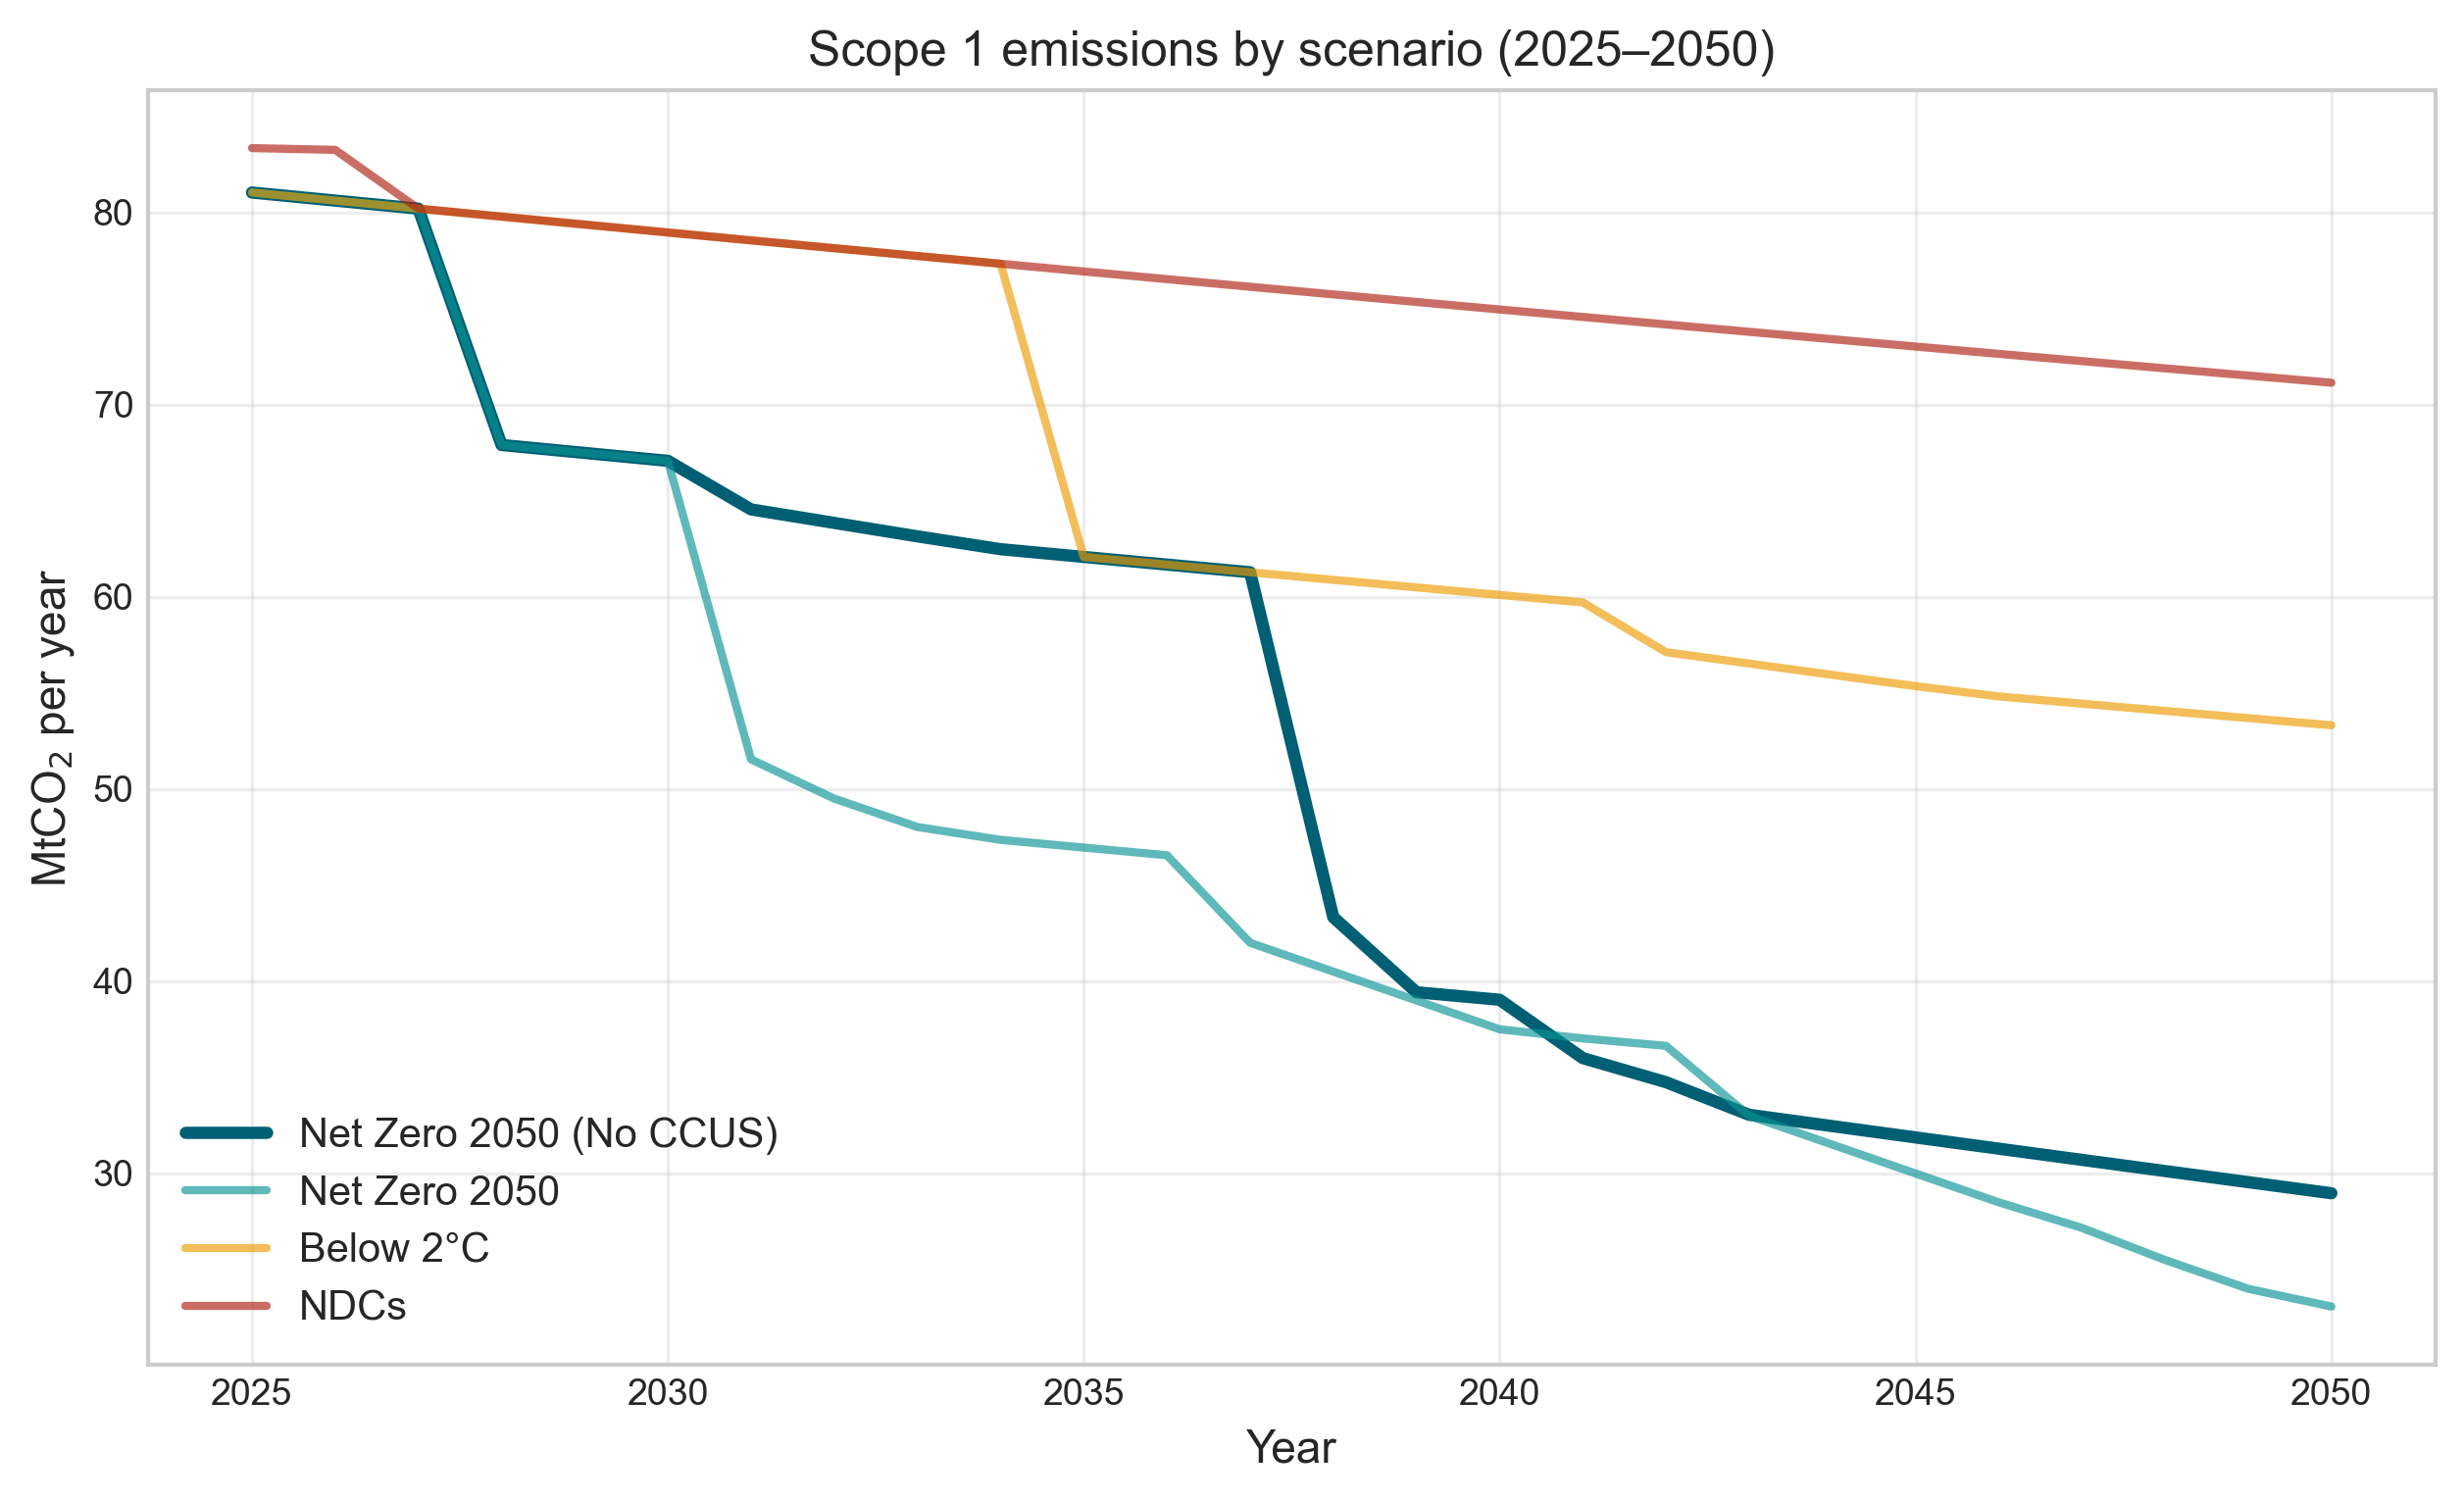
\includegraphics[width=0.8\linewidth]{scope1_by_scenario}
  \caption{Scope~1 emissions by scenario, including the Net Zero 2050 pathway with CCUS disabled (2025--2050).}
  \label{fig:scope1-by-scenario}
\end{figure}

\subsection{High carbon prices are the only trigger for low-carbon technologies}

The annual production mix in Table~\ref{tab:annual-shares-ngfs_netzero2050} and Figure~\ref{fig:technology-transition} shows that technology switching is tightly coupled to discrete carbon-price thresholds. Scrap-based EAF deployment remains frozen at 4.5\% of output while allowance prices stay below \$100/tCO$_2$, then leaps to 22.8\% in 2028 once the Net Zero pathway clears \$110/tCO$_2$. That jump reflects a single 9~Mt capacity tranche because POSCO must construct entirely new EAF modules—its present operations are almost exclusively blast-furnace based, with only niche stainless EAF assets totalling 1.7~Mt/y that cannot substitute for automotive-grade flat products \citep{POSCO2023SR}. Scrap availability then caps electrification at 35.7\% even under the most aggressive prices. The stacked panels in Figure~\ref{fig:technology-transition} translate the long tables into time-series shares, with the top frame emphasising the Net Zero 2050 (No CCUS) sensitivity.

Carbon capture enters only after prices reach \$165/tCO$_2$ in 2031. At that point the model retrofits one 9~Mt module, and subsequent price rises to \$225 and \$255/tCO$_2$ trigger further retrofits until CCUS-equipped furnaces supply 51\% of 2050 production. Lower trajectories never activate capture: Below~2$^\circ$C pricing stalls at \$240/tCO$_2$ and therefore leaves 64\% of output unabated blast furnaces, while the NDC-consistent ceiling of \$100/tCO$_2$ fails to justify any structural change and keeps the BF--BOF share above 95\% throughout (see Tables~\ref{tab:annual-shares-ngfs_below2c} and \ref{tab:annual-shares-ngfs_ndcs}). In other words, only sustained prices well above \$150/tCO$_2$ unlock capital-intensive decarbonisation routes.

Hydrogen-based direct reduction, FINEX, and natural-gas DRI remain dormant across scenarios because levelised costs stay higher than the CCUS-plus-scrap blend even at \$450/tCO$_2$. Our assumed hydrogen costs (\$4.5/kg in 2030, falling to \$2.5/kg by 2050) align with techno-economic reviews \citep{MaterialEconomics2019,demailly2018european} that place the breakeven for early hydrogen steel below \$2.0--\$2.5/kg. Without such cost breakthroughs, carbon pricing alone cannot make hydrogen competitive within the 2025--2050 horizon.

\begin{figure}[!t]
  \centering
  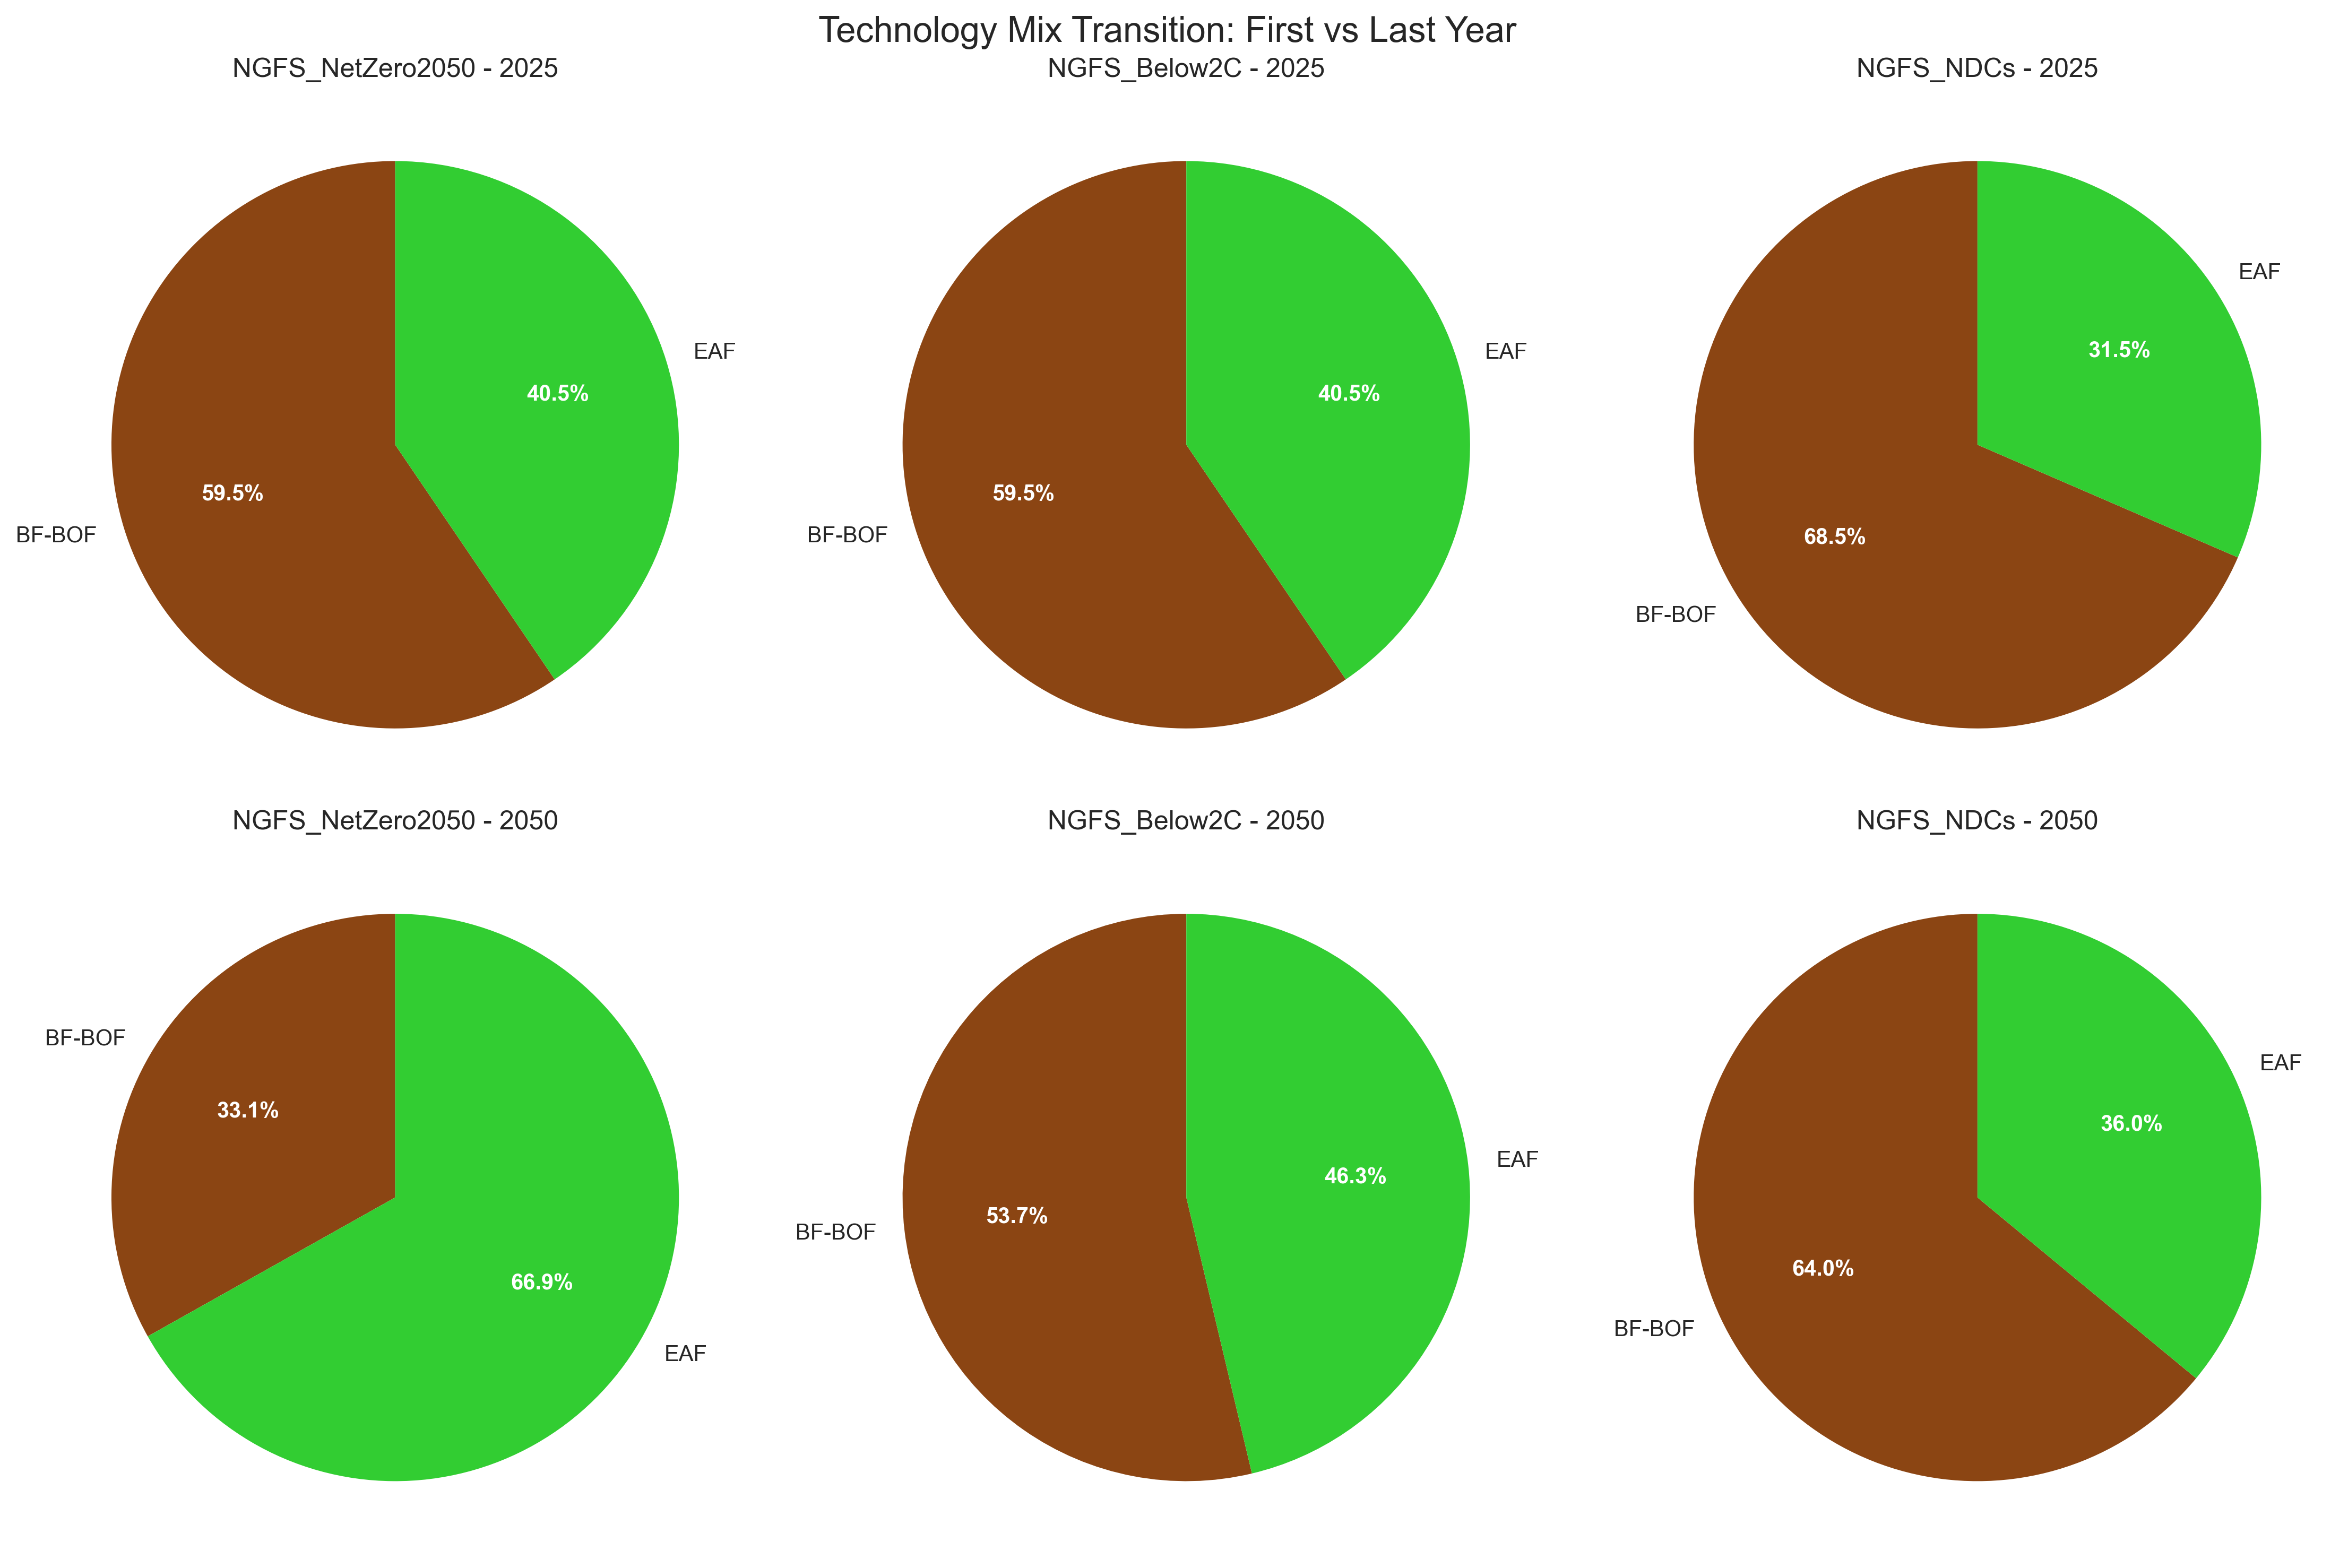
\includegraphics[width=0.8\linewidth]{technology_transition}
  \caption{Technology shares by scenario. The top panel emphasises the Net Zero 2050 pathway with CCUS disabled; lower panels show the NGFS Net Zero, Below~2$^\circ$C, and NDC trajectories.}
  \label{fig:technology-transition}
\end{figure}

\begin{figure}[!t]
  \centering
  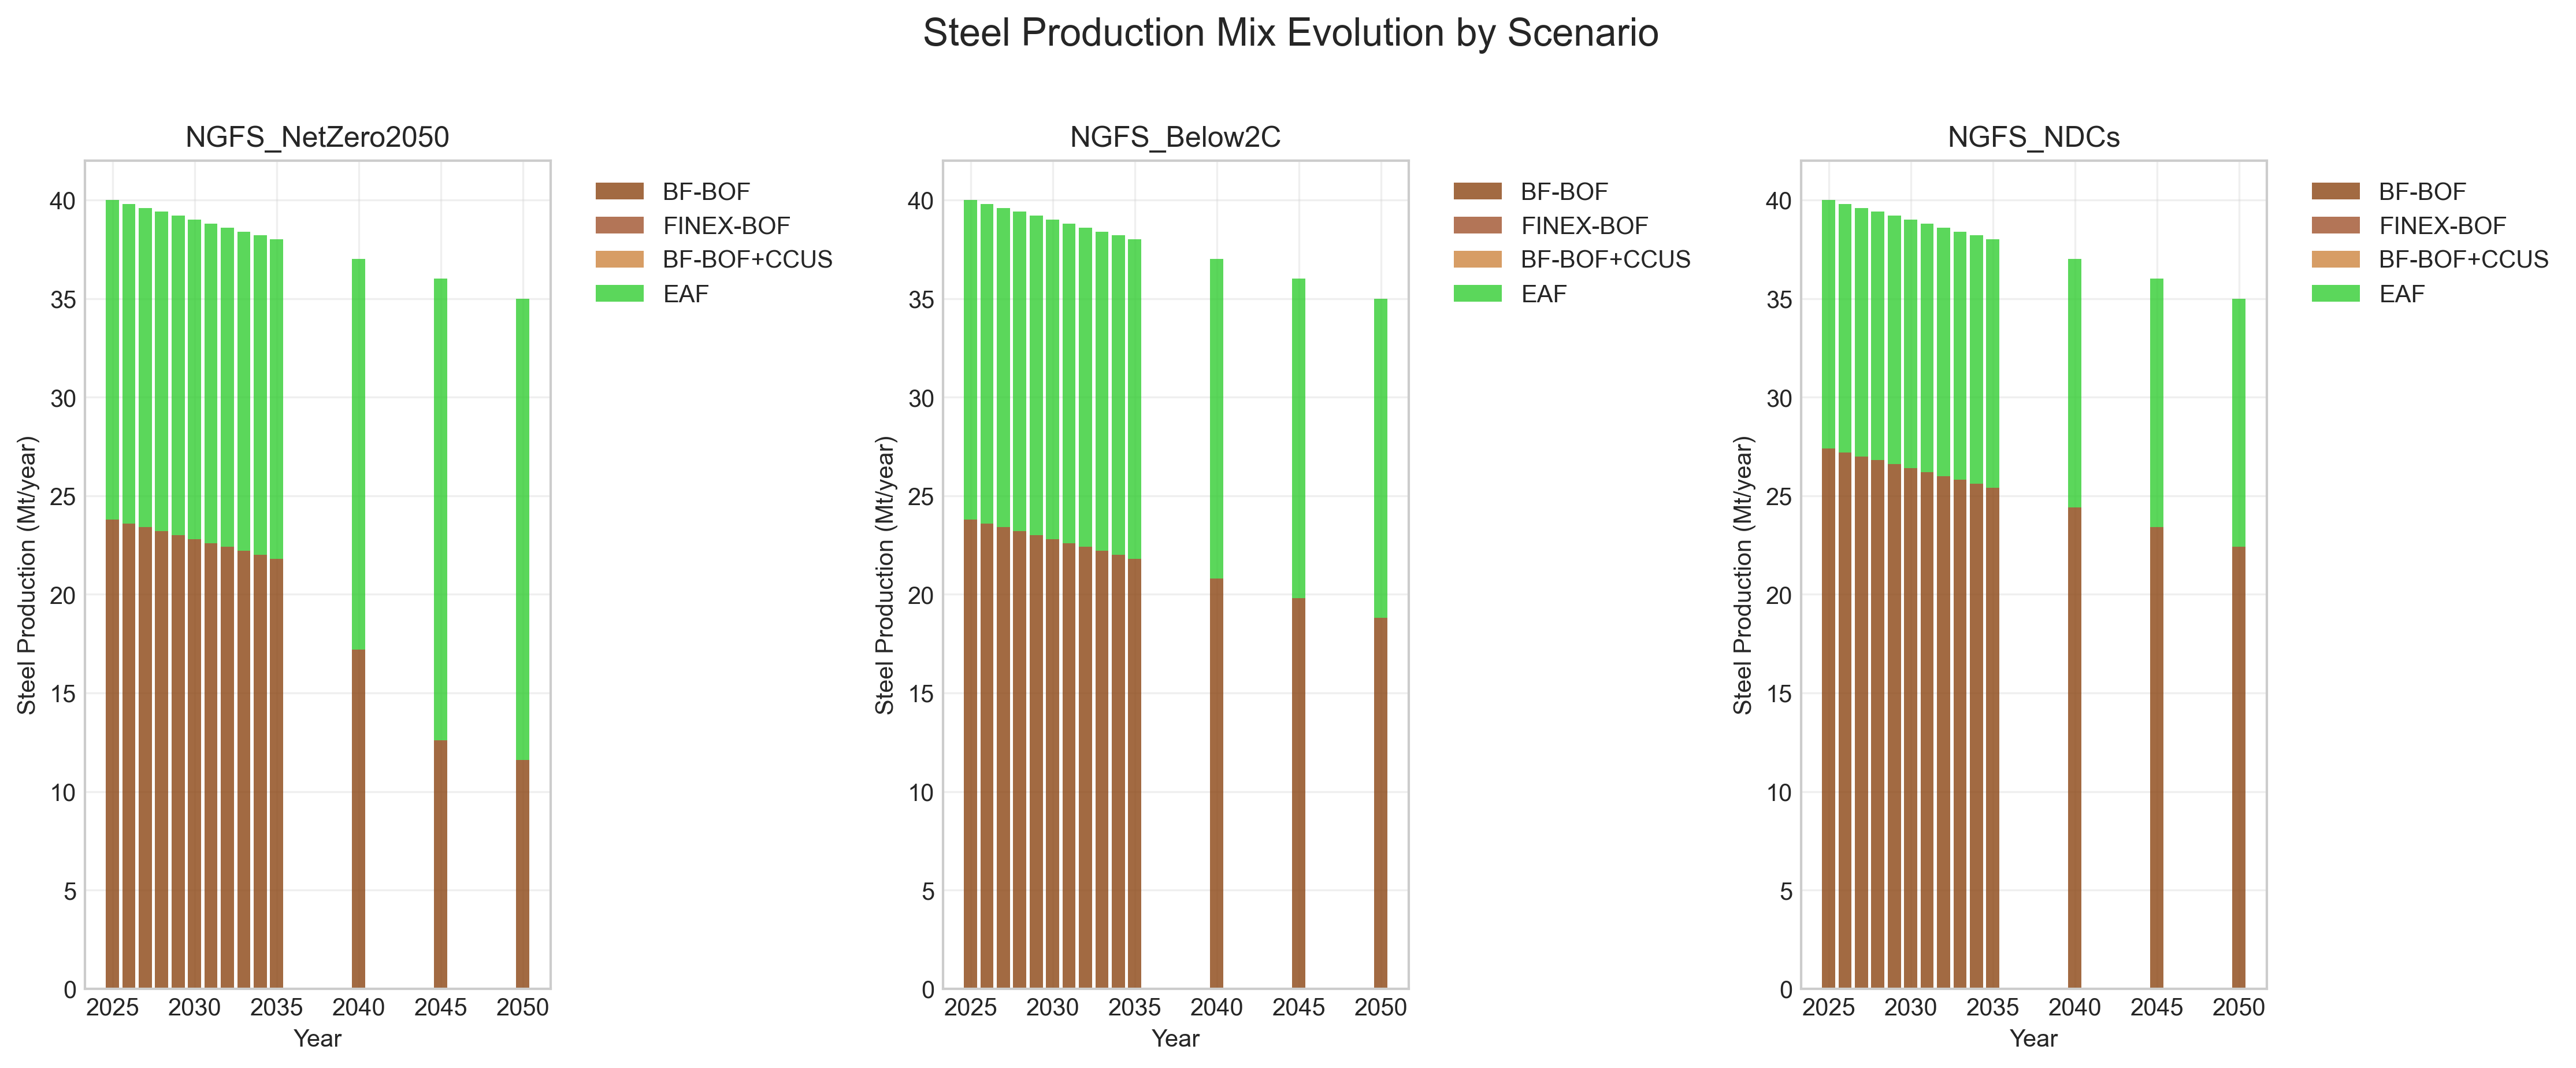
\includegraphics[width=0.8\linewidth]{production_mix_evolution}
  \caption{Production mix by technology route (Mt/year). Panels mirror Figure~\ref{fig:technology-transition}, with the Net Zero 2050 (No CCUS) case highlighted.}
  \label{fig:production-mix}
\end{figure}

\subsection{Carbon budget compliance still fails without stronger prices}

Integrating annual emissions produces cumulative totals of 1{,}190~MtCO$_2$ (Net Zero), 1{,}713~MtCO$_2$ (Below~2$^\circ$C), and 1{,}981~MtCO$_2$ (NDCs) over 2025--2050. Compared with POSCO's 1{,}110~MtCO$_2$ allocation, the Net Zero scenario still overshoots by 79.6~MtCO$_2$ (+7.2\%), while Below~2$^\circ$C exceeds the budget by 603~MtCO$_2$ (+54\%) and the NDC trajectory by 871~MtCO$_2$ (+78\%). The cumulative gap therefore maps directly into a carbon-price gap: the difference between the NDC ceiling (\$100/tCO$_2$) and the Net Zero peak (\$450/tCO$_2$) yields a 791~MtCO$_2$ reduction, implying that the residual 80~MtCO$_2$ shortfall would require prices rising well above \$450/tCO$_2$ absent new constraints on production. Persistent free-allocation coverage exacerbates the problem: even under Net Zero, only 72~MtCO$_2$ of cumulative emissions are ETS-liable, and the Below~2$^\circ$C path pays for just 596~MtCO$_2$ out of 1,713~MtCO$_2$ emitted. Closing the residual gap under Net Zero therefore requires either a sharper price floor escalation after 2040 or a faster phase-down of free allocation so that firms internalise carbon costs before the next blast-furnace relining cycle. Detailed calculations are provided in \texttt{outputs/analysis/carbon\_budget\_compliance.csv}.

\begin{figure}[!t]
  \centering
  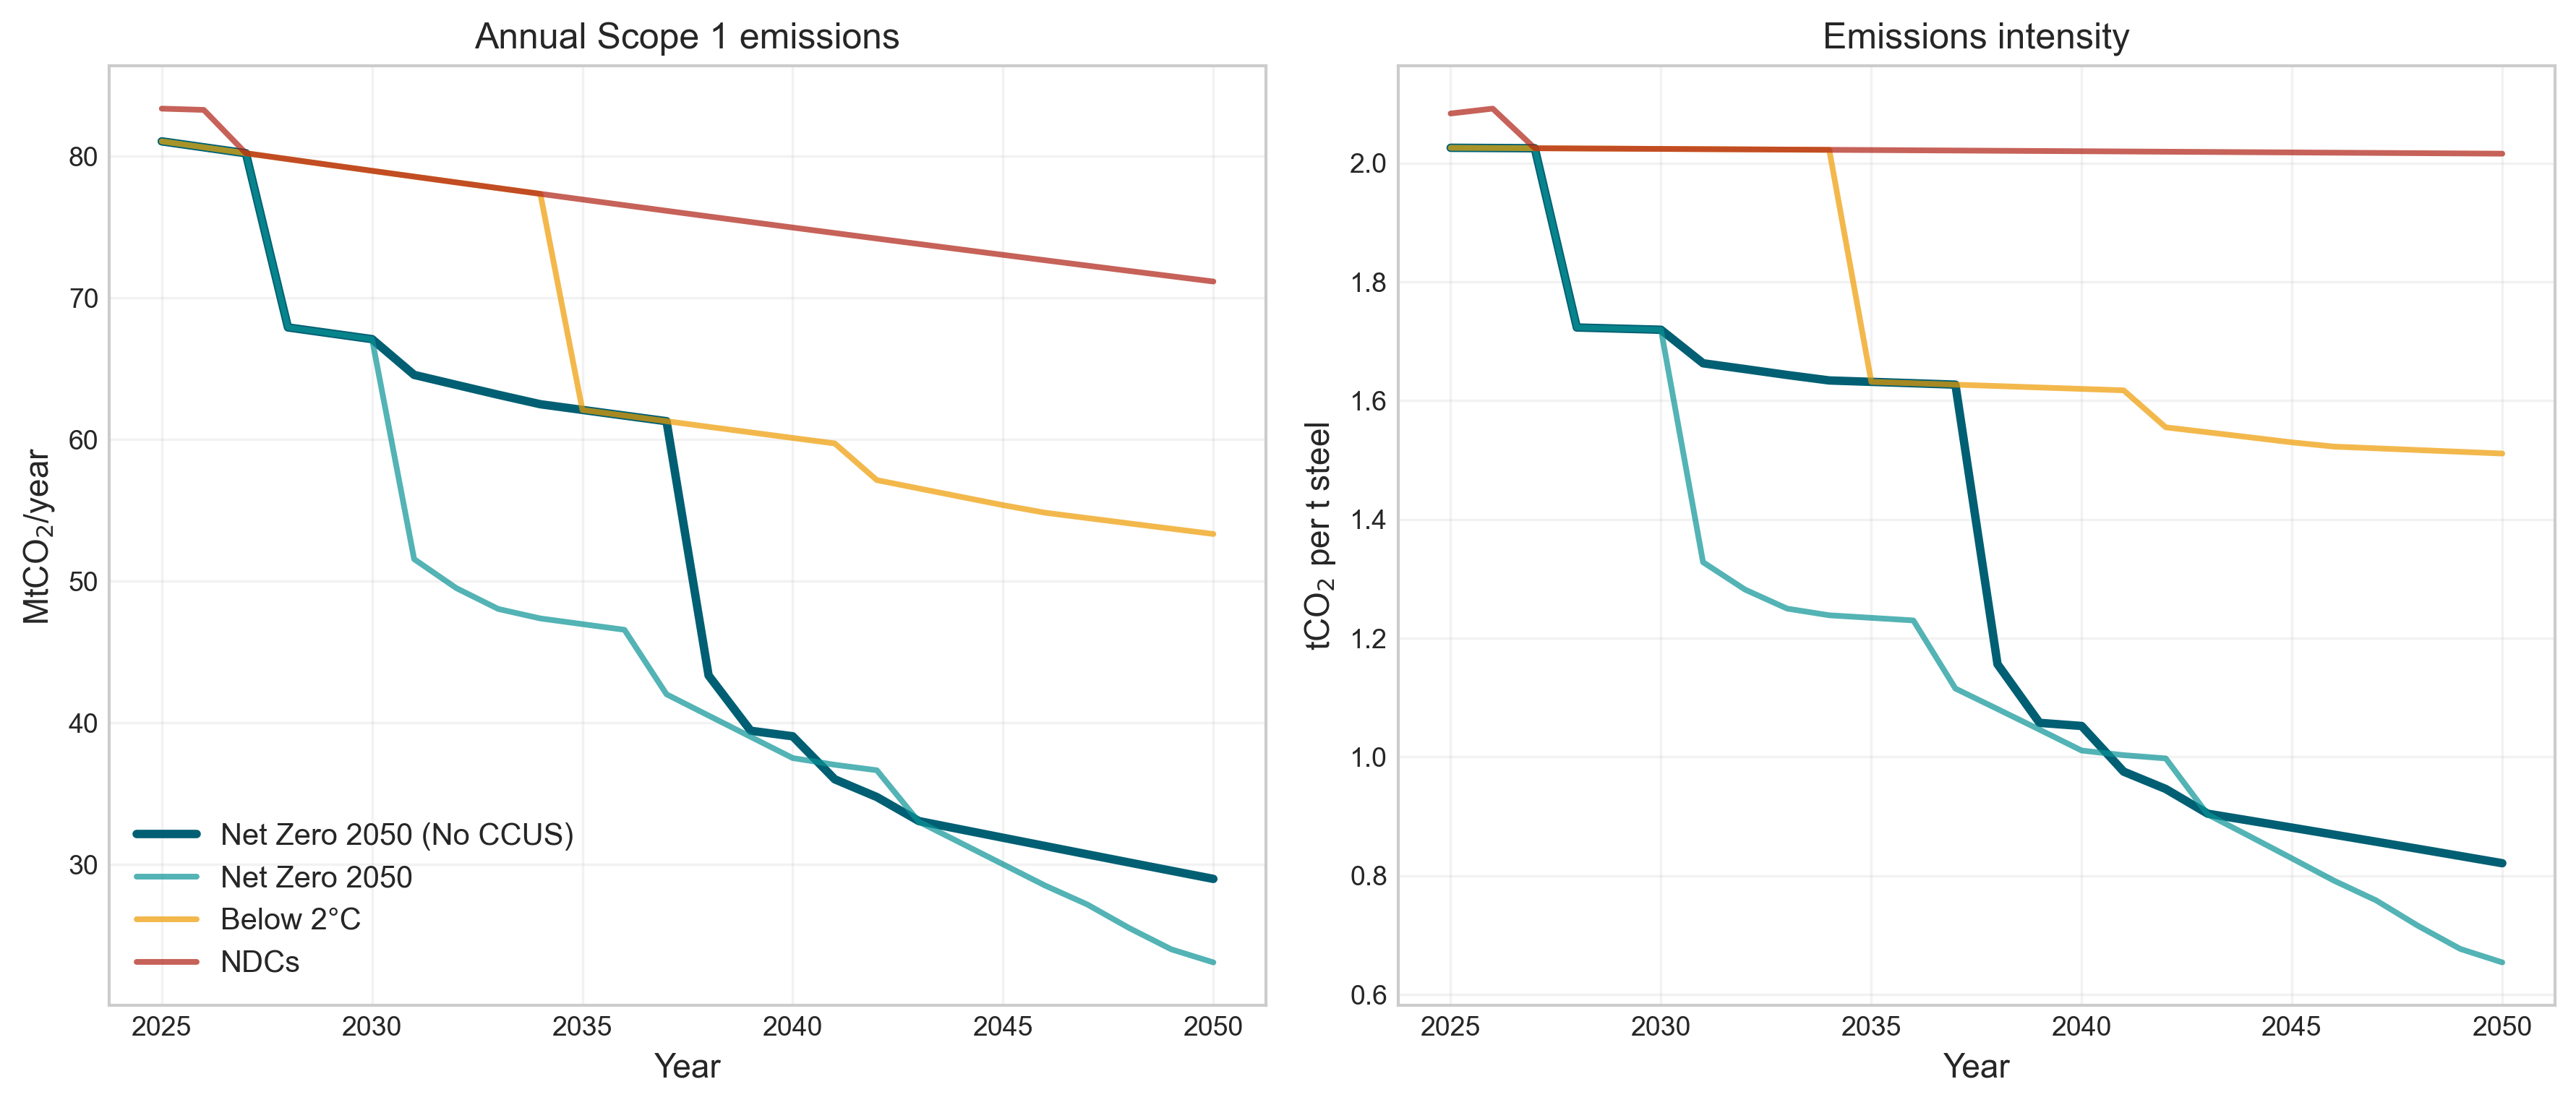
\includegraphics[width=0.85\linewidth]{emissions_pathways}
  \caption{Annual Scope~1 emissions (left) and emissions intensity (right) by scenario.}
  \label{fig:emissions-pathways}
\end{figure}

Figure~\ref{fig:emissions-pathways} shows that only the NGFS Net Zero pathways materially shift emissions intensity; the no-CCUS sensitivity keeps intensity above 0.8~tCO$_2$/t even in 2050, reflecting the residual reliance on hydrogen-fed DRI and unabated blast furnaces.

\subsection{Cost structure shifts from compliance spending to capital turnover}

Summing undiscounted expenditure over 2025--2050 shows that the Net Zero pathway still delivers the lowest lifetime system cost: \$791~billion versus \$871~billion (Below~2$^\circ$C) and \$842~billion (NDCs). Dividing by cumulative steel output (978~Mt) yields average costs of \$810/t under Net Zero, \$891/t under Below~2$^\circ$C, and \$861/t in the compliance-heavy NDC case. The divergence is driven by ETS exposure. NDC pricing leaves 863~MtCO$_2$ of net ETS-liable emissions and \$59.7~billion in compliance payments (7.1\% of lifetime outlays). Net Zero pricing still emits 1,190~MtCO$_2$, but only 72~MtCO$_2$ is ETS-liable, trimming payments to \$9.3~billion (1.2\% of cost) and redirecting cashflow toward CCUS retrofits and electrification upgrades, whereas disabling capture under the same price path lifts liabilities to 206~Mt and payments to \$43~billion (Figure~\ref{fig:ets-costs}). Table~\ref{tab:cost-abatement} shows that ambition beyond the NDC baseline is cost saving in the Net Zero case (minus \$64/tCO$_2$) but requires positive \$108/tCO$_2$ support for the intermediate Below~2$^\circ$C pathway. Ambitious pricing therefore swaps recurring ETS fees for front-loaded low-carbon investment, consistent with the investment-switching logic in \citet{fowlie2016carbon}.

\begin{figure}[!t]
  \centering
  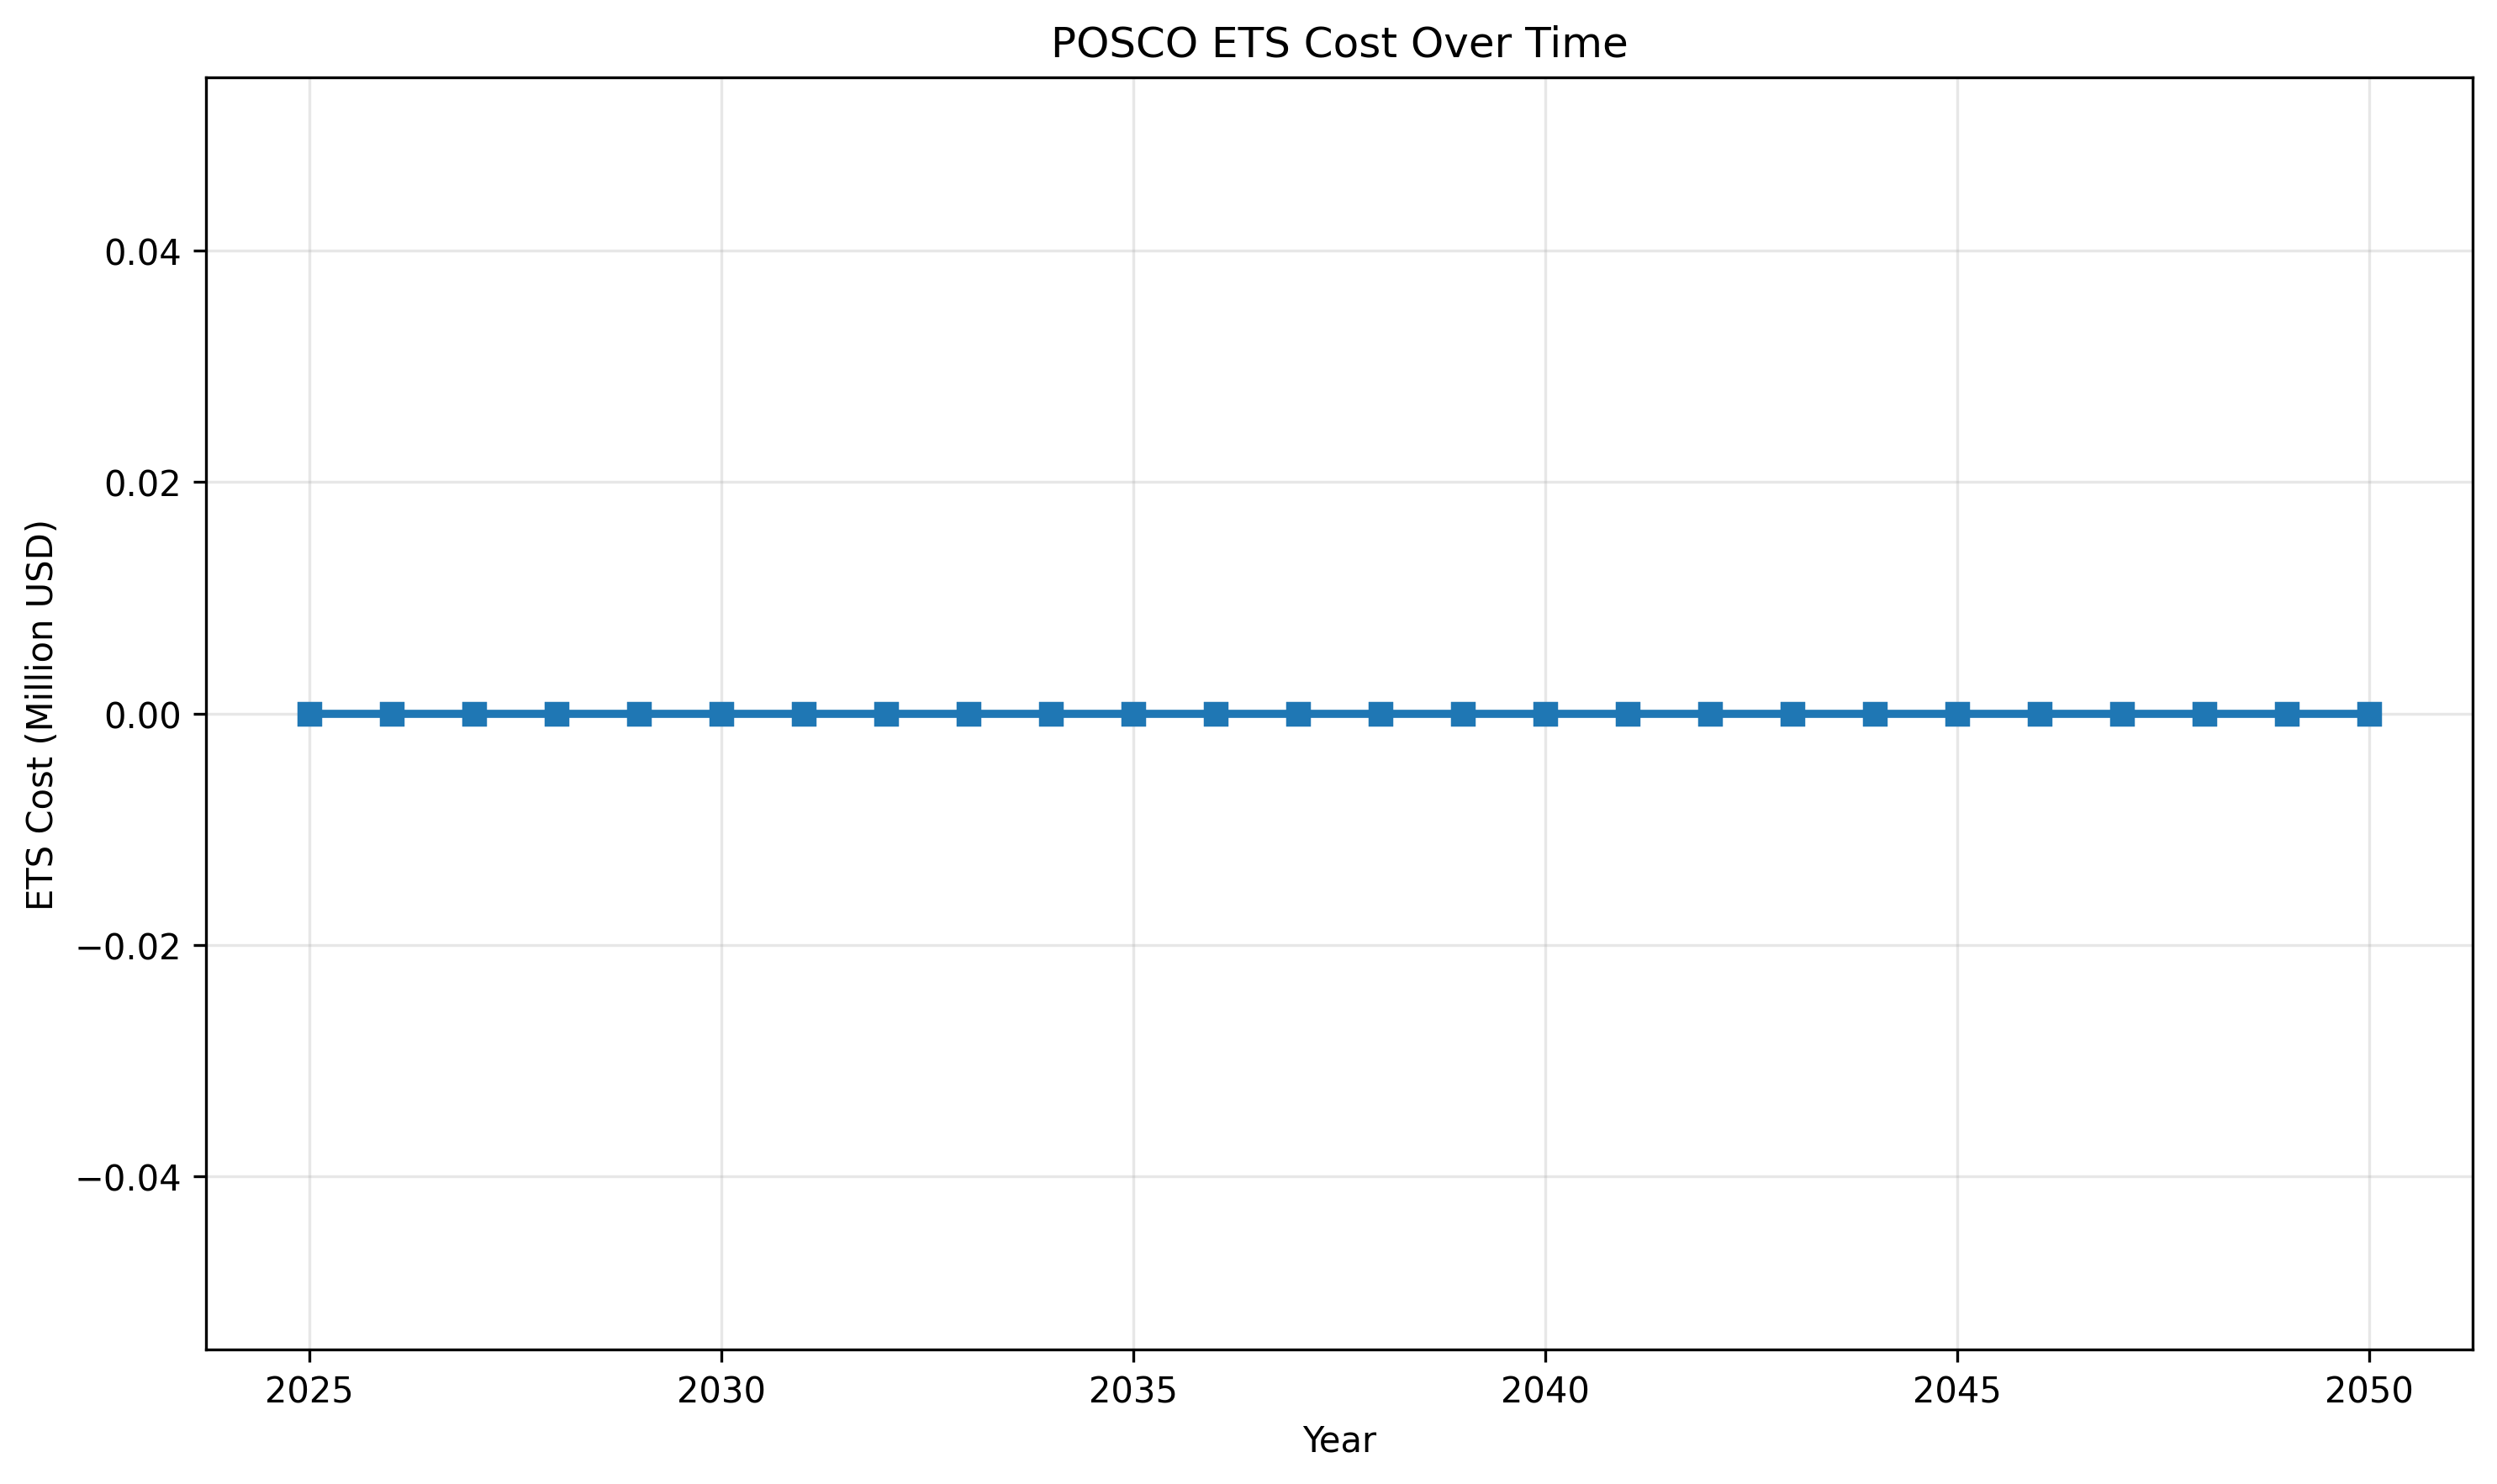
\includegraphics[width=0.8\linewidth]{ets_cost_by_scenario}
  \caption{Annual ETS compliance costs across the NGFS price trajectories plus the Net Zero 2050 (No CCUS) sensitivity.}
  \label{fig:ets-costs}
\end{figure}

\begin{figure}[!t]
  \centering
  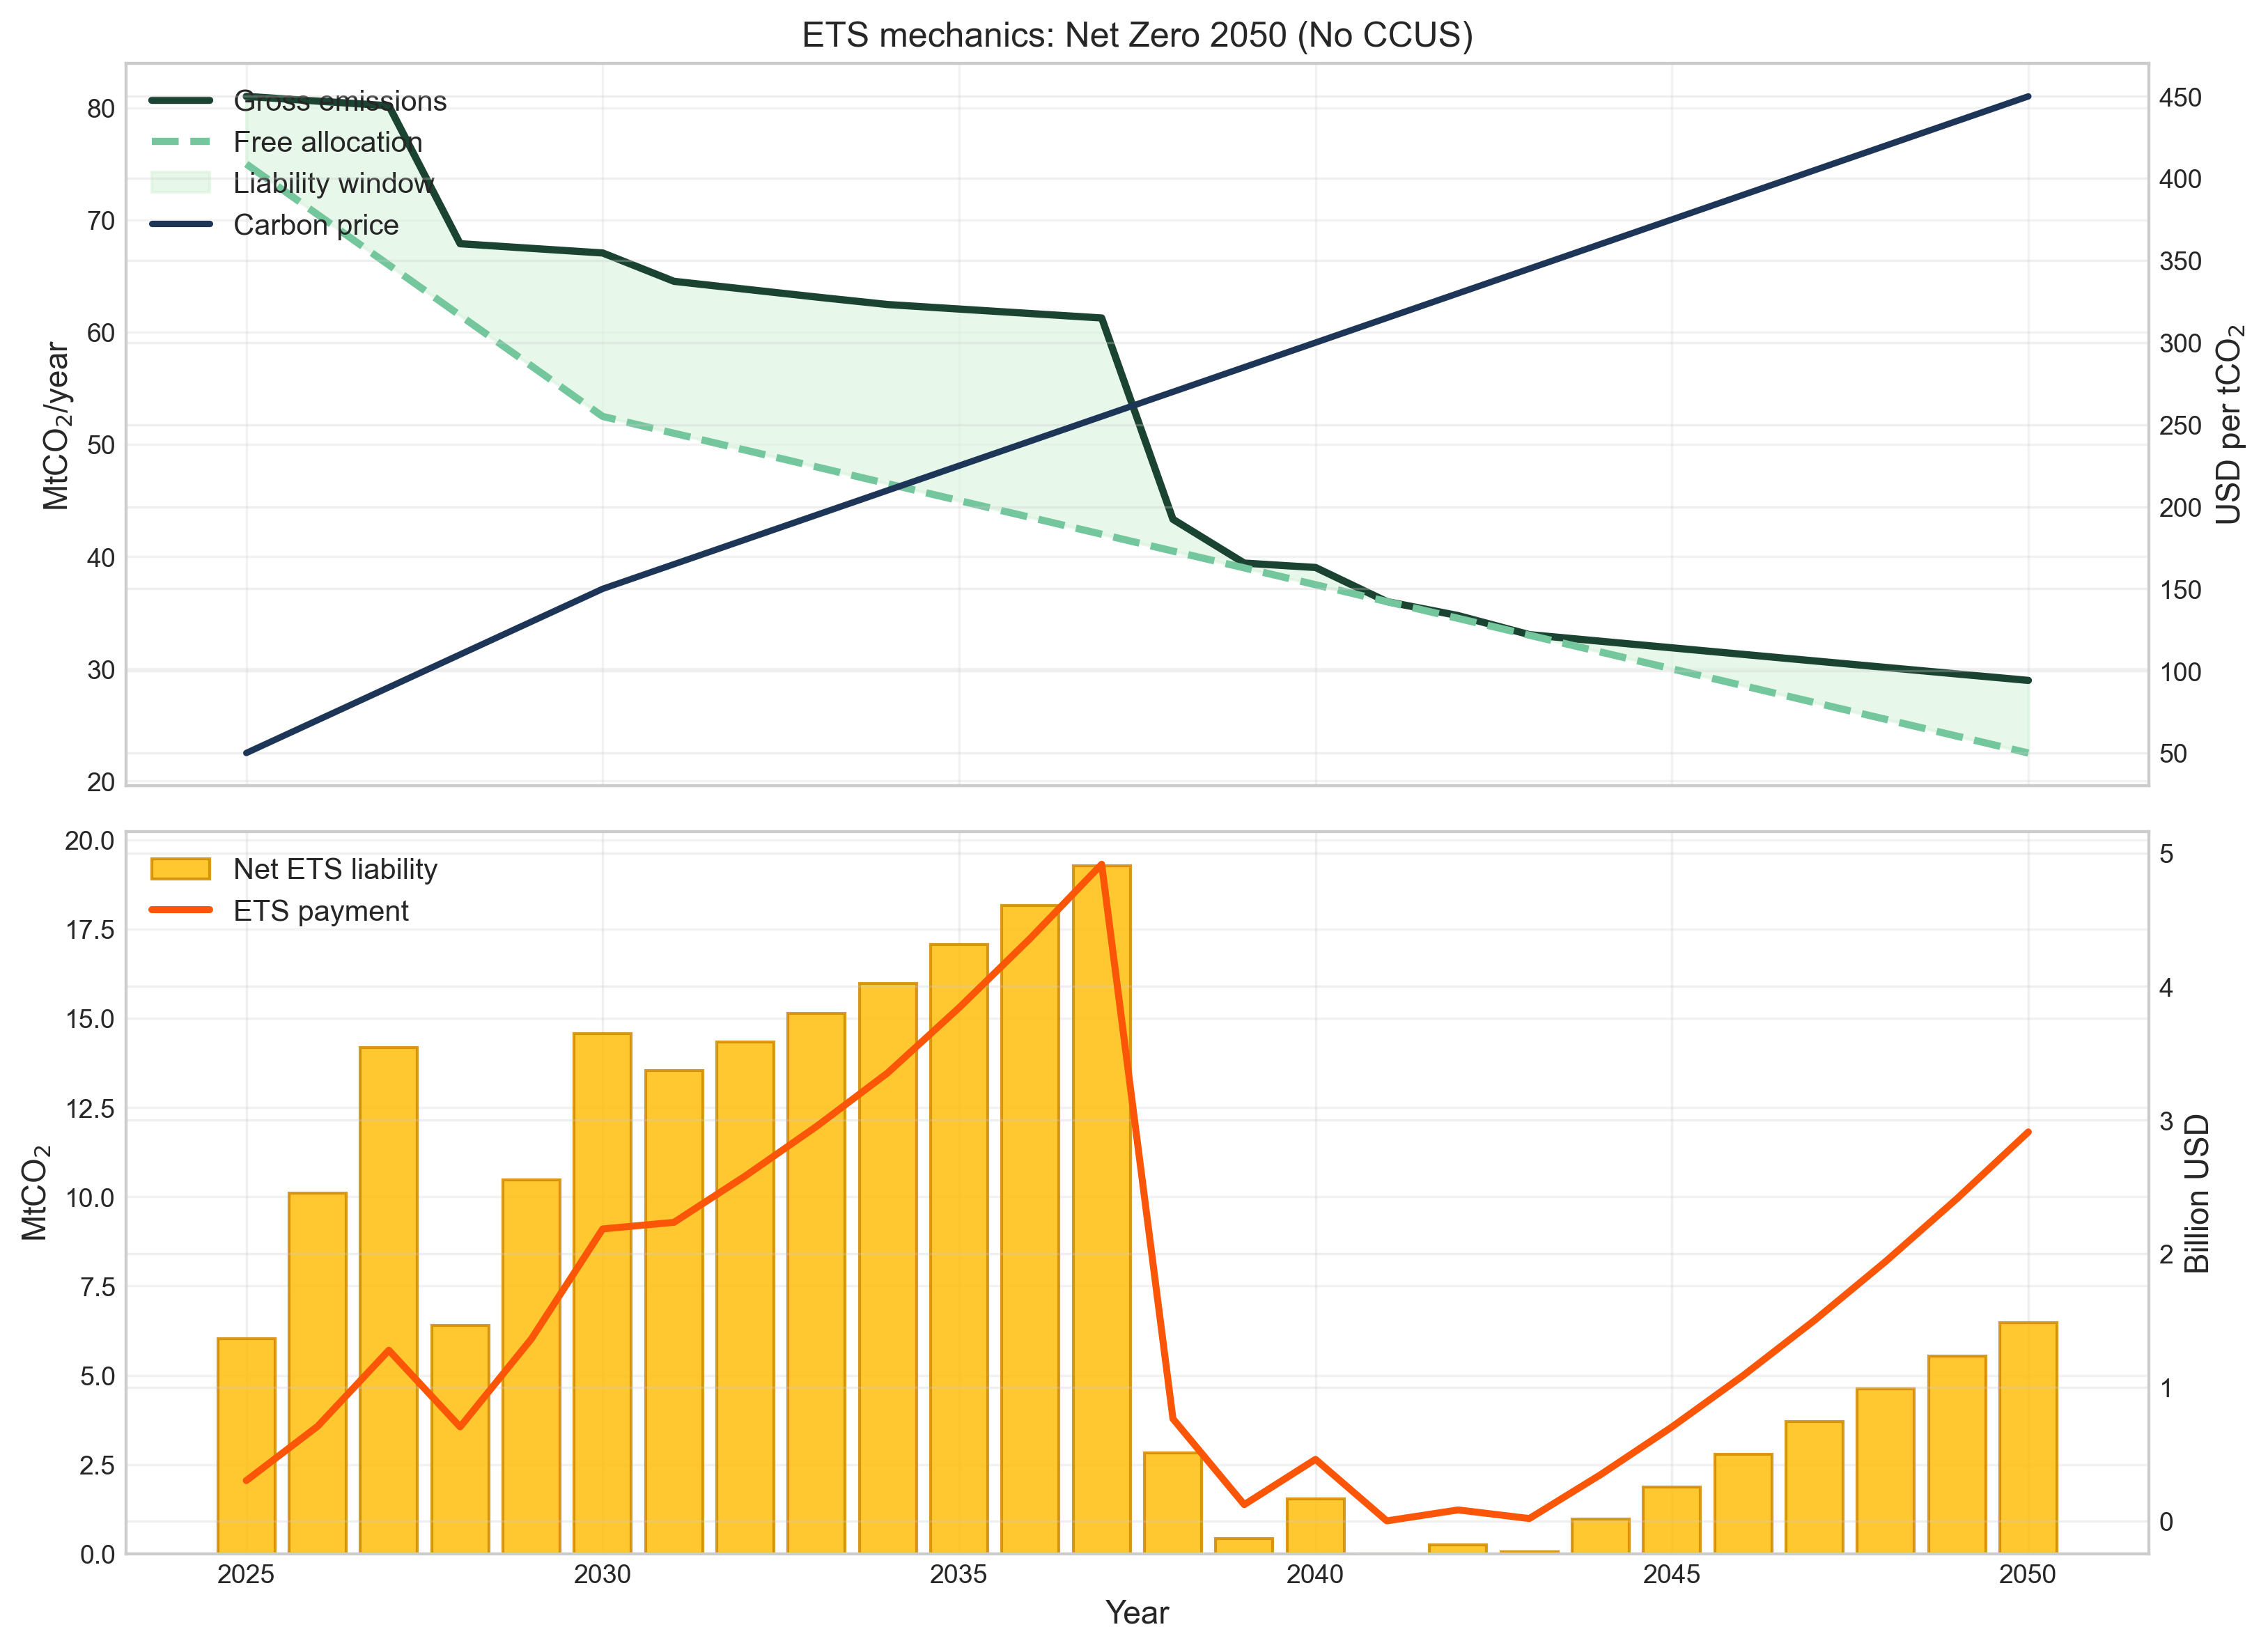
\includegraphics[width=0.85\linewidth]{ets_cost_logic}
  \caption{ETS cost mechanics for the Net Zero 2050 (No CCUS) pathway. The top panel contrasts gross emissions, free allocation, and allowance prices; the lower panel shows net ETS liabilities and resulting payments.}
  \label{fig:ets-logic}
\end{figure}

Figure~\ref{fig:ets-logic} clarifies how the compliance bill escalates once capture is unavailable. The free-allocation schedule falls faster than gross emissions after 2030, reopening a liability window that widens as allowance prices cross \$150/tCO$_2$. By the mid-2030s the liability volumes exceed 5~MtCO$_2$/year and, combined with \$200--\$300/tCO$_2$ prices, generate multi-billion-dollar payments that mirror the quadrupling reported above.

\subsection{Implications for competitiveness}

Expressed per ton of crude steel, average costs fall from \$861/t under the NDC pathway to \$810/t under Net Zero because avoided ETS fees outweigh the higher capital spend on CCUS and electric-melt upgrades. That \$51/t differential sits within the expected range of European Union Carbon Border Adjustment Mechanism (CBAM) levies (EUR~50--100/tCO$_2$), implying that Korean exports could remain competitive if domestic carbon price reforms are synchronised with border adjustment mechanisms \citep{Vogl2018}. Yet the optimal portfolio is now split between CCUS-equipped hot metal (51\%) and scrap-based EAF (36\%). This raises execution risks around capture performance, storage deployment, and sustained scrap supply chains despite the absence of hydrogen uptake in the baseline. Targeted support for CO$_2$ transport and storage infrastructure, high-grade scrap collection, and quality assurance therefore becomes critical to lock in the cost advantage highlighted by the model \citep{Griffin2020}.

\subsection{Sensitivity analysis: hydrogen costs and CCUS availability}

To test the robustness of these findings, we re-ran the Net Zero pathway under three alternative hydrogen cost assumptions bundled with the repository (\texttt{outputs/h2\_breakthrough}, \texttt{h2\_optimistic}, and \texttt{h2\_zero}). Lowering delivered hydrogen prices from the baseline \$4.5/kg to a ``breakthrough'' trajectory consistent with \$2.5/kg in 2035 barely shifts the technology mix: scrap-EAF rises to 46\% of 2050 output, CCUS-backed blast furnaces fall to 38\%, and hydrogen-based DRI still fails to enter. Cumulative emissions are essentially unchanged at 1{,}190~MtCO$_2$, and lifetime system costs move by less than \$1.5~billion. Even the extreme ``zero-cost hydrogen'' stress test yields the same outcome, underscoring that capital intensity, ore quality constraints, and scrap ceilings---rather than molecule prices alone---keep hydrogen routes out of the optimal portfolio. These sensitivities confirm that policy packages aimed solely at subsidising hydrogen would leave the carbon-budget gap intact unless paired with infrastructure that tackles the non-price frictions identified above.

We also disable CCUS entirely by setting the capture rate to zero while maintaining the NGFS Net Zero carbon prices. The resulting portfolio swings toward hydrogen direct-reduced iron: H$_2$ routes capture 35.7\% of production by 2050, scrap-EAF remains capped at 35.3\%, and unabated blast furnaces supply the remaining 29.0\%. Yet the emissions outcome deteriorates markedly. Cumulative Scope~1 emissions climb to 1{,}324~MtCO$_2$ (+19\% versus the budget), 2050 emissions settle at 29.0~MtCO$_2$, and net ETS liabilities quadruple to 206~Mt, lifting cumulative ETS payments to \$43~billion (Table~\ref{tab:scenario-comparison}). Average steelmaking costs increase to \$815/t, eroding much of the competitiveness gain delivered by CCUS-equipped Net Zero pathways. The no-CCUS sensitivity therefore shows that hydrogen uptake at current price trajectories requires capture to absorb residual blast-furnace output; without a credible CCUS programme, the ETS would shoulder far larger compliance volumes and the carbon-budget gap would remain unacceptably wide.

\section{Discussion}

Our empirical results highlight a persistent adequacy gap between Korea's announced carbon price trajectory and the incentives required for POSCO to remain within its sectoral carbon budget. Because the optimization retains robust profits for the firm in every scenario, the shortfall is not technological but institutional: price signals remain too low, and free allocation continues to mute marginal abatement incentives.

\subsection{The carbon pricing adequacy gap}

Three findings stand out. First, even the NGFS Net Zero schedule leaves a 80~MtCO$_2$ overshoot, demonstrating that current plans to lift allowance prices to \$250/tCO$_2$ by 2050 are necessary but still insufficient for budget compliance while free allocation dulls marginal incentives. Second, the optimisation now leans heavily on CCUS retrofits (51\% of 2050 output) alongside a capped scrap share of 36\%, revealing that investment-grade capture, storage, and scrap logistics have to materialise for the price signal to bite. When CCUS is switched off altogether, cumulative emissions jump to 1,324~MtCO$_2$ (+19\%), hydrogen DRI captures 36\% of output, and cumulative ETS payments balloon to \$43~billion, confirming that Net Zero prices alone cannot compensate for missing capture infrastructure. Third, the NDC trajectory's 871~MtCO$_2$ overshoot confirms that a “wait-and-see” price path locks in high-carbon assets for another investment cycle, echoing concerns raised in ex-post evaluations of the EU ETS \citep{Green2021, martin2016industry}.

\subsection{Institutional and political economy barriers}

Why does Korea continue to under-price carbon despite ambitious net-zero rhetoric? The K-ETS still distributes the majority of allowances for free to energy-intensive trade-exposed firms, including POSCO \citep{kim2021kets, ICAP2024}. Free allocation functions as an implicit production subsidy that dampens the marginal benefit of abatement \citep{neuhoff2012inclusion}. Moreover, industrial policy has concentrated on headline hydrogen demonstrations and plant-level CCUS pilots while under-investing in the enabling systems that determine model outcomes: nationwide scrap recovery, CO$_2$ transport and storage hubs, and low-carbon power contracts. CCUS only scales in the optimisation because it is assumed that such infrastructure exists. Without reforms to the allocation regime and supportive infrastructure for both circular steelmaking and carbon storage, political economy pressures to protect incumbent blast furnaces will continue to dominate \citep{MaterialEconomics2019}.

\subsection{Policy package for credible alignment}

Aligning carbon pricing with the steel-sector budget therefore requires a broader package than price escalation alone. Table~\ref{tab:policy-matrix} summarises the priority measures. First, Korea should adopt a binding allowance price floor that tracks the NGFS Net Zero schedule but escalates more steeply after 2040, providing the missing commitment device highlighted by \citet{fowlie2016carbon}. Second, free allocation must be phased down faster than currently planned—at least 5--7 percentage points per year after 2025—so that firms begin to pay the full marginal cost of emissions before major reinvestment decisions in the early 2030s. Third, complementary industrial policies should focus on de-risking both scrap-based electrification and carbon capture: nationwide scrap collection standards, low-cost industrial power tariffs linked to renewable build-out, and credit guarantees for EAF and CCUS retrofits would ensure that the cost-effective pathway identified by the model remains politically feasible. Fourth, the government should introduce carbon contracts for difference (CCfDs) that guarantee a strike carbon price for abatement investments, bridging the gap between uncertain ETS revenues and the levelised cost of CCUS and hydrogen-ready assets \citep{Neuhoff2019CCfD,Richstein2017CCfD}. Finally, targeted hydrogen and CCUS funding should be conditional on clear cost-reduction milestones; otherwise, scarce public resources risk supporting technologies that remain outcompeted by circular production routes.

% ===== 6. Limitations and future work =====
\section{Limitations}\label{sec:limitations}

While this study provides detailed insights into POSCO's optimal decarbonization pathways, several limitations should be acknowledged. First, the model assumes perfect foresight regarding technology costs, carbon prices, and demand trajectories, which may not reflect real-world decision-making under uncertainty. Second, the analysis focuses on a single firm and may not capture broader industry dynamics, including competition effects, supply chain interactions, and technology spillovers across Korean steel producers. Third, the demand pathway is treated as exogenous, whereas carbon pricing and technology transitions could endogenously affect steel consumption patterns through price pass-through and material substitution.

The model also abstracts from several technical and regulatory complexities. Blast furnace relining schedules are approximated rather than explicitly modeled, potentially affecting the precise timing of capacity retirements. Product quality constraints between routes are simplified, and the analysis excludes Scope 3 emissions and lifecycle impacts of hydrogen production. CCUS performance is represented by a deterministic 80\% capture rate with full transport and storage readiness; real-world deployment risk, reservoir availability, and monitoring obligations could materially change the cost and emissions outcomes, so the CCUS-heavy Net Zero portfolio should be interpreted as contingent on aggressive infrastructure delivery. Finally, the study does not model potential complementary policies such as green procurement standards, R\&D subsidies, or international carbon border adjustments, which could significantly alter the investment landscape.

% ===== 7. Conclusion =====
\section{Conclusion}

This study provides the first quantitative test of whether Korea's carbon pricing trajectory can align POSCO's investment incentives with the steel-sector carbon budget implied by national climate commitments. The answer is sobering: even under the NGFS Net Zero 2050 pathway, residual overshoots persist because current policy settings combine rising nominal prices with extensive free allocation and limited support for the most cost-effective abatement options.

\subsection{Key empirical findings}

Three empirical results stand out. First, carbon pricing reduces emissions sharply but not sufficiently: cumulative Scope~1 emissions fall from 1{,}981~MtCO$_2$ in the NDC trajectory to 1{,}190~MtCO$_2$ under Net Zero, yet the latter still exceeds POSCO's 1{,}110~MtCO$_2$ budget by 80~MtCO$_2$ (+7\%). Second, the cost-minimising transition now relies on a blended portfolio of CCUS-equipped blast furnaces (51\% of 2050 output) and scrap-based electric arc furnaces (36\%), while hydrogen routes never enter at current cost assumptions—unless CCUS is unavailable, in which case hydrogen DRI expands to 36\% of output but cumulative emissions surge to 1{,}324~MtCO$_2$. Third, ambitious pricing improves cost competitiveness instead of eroding it: average steel production costs decline from \$861/t in the NDC scenario to \$810/t under Net Zero because firms substitute capital expenditure for recurring ETS payments.

\subsection{Policy implications}

These findings call for a step change in the design of the Korean Emissions Trading System. Raising the allowance price ceiling alone will not deliver budget compliance if allowances continue to be distributed for free. Policy priorities should therefore include: (i) a binding price floor that overtly targets \emph{at least} \$500/tCO$_2$ by the mid-2040s—above the NGFS Net Zero trajectory—to activate the final CCUS tranche identified in Table~\ref{tab:annual-shares-ngfs_netzero2050}; (ii) an accelerated phase-out of free allocation so that steel producers face full marginal carbon costs before the next blast-furnace relining cycle; and (iii) industrial policies that de-risk large-scale scrap collection, CO$_2$ transport and storage, and low-cost electricity supply for both EAFs and capture units. In parallel, hydrogen and CCUS support should be tied to transparent cost benchmarks to avoid subsidising technologies that remain outcompeted by circular production routes.

\subsection{Broader implications}

The Korean steel sector illustrates a wider lesson for industrial decarbonisation: credible climate policy must combine high and predictable carbon prices with institutional reforms that transmit those prices to investment decisions. Without such reforms, even apparently ambitious trajectories leave large policy-performance gaps that threaten national climate credibility. The analytical framework developed here can be applied to other energy-intensive sectors to benchmark carbon pricing adequacy against sectoral budgets and to prioritise complementary measures that turn price signals into tangible investment shifts. In practice, pairing stronger ETS instruments with CCfDs that underwrite early low-carbon steel production offers the clearest route to reconciling investment risk with the steep decarbonisation commitments facing primary steelmakers \citep{Neuhoff2019CCfD}.

% ===== Tables =====
\begin{table}[ht]
  \centering
  \caption{Key model assumptions and baseline parameter values (real USD 2024)}
  \label{tab:assumptions}
  \begin{threeparttable}
  \begin{tabular}{@{}llc@{}}
    \toprule
    Category & Parameter & Value/Path \\
    \midrule
    \multirow{3}{*}{Economic} & Discount rate ($\rho$) & 5\% (baseline); 3\% (sensitivity) \\
    & Capacity utilization ($\mu$) & 90\% maximum \\
    & Model horizon & 2025--2050 (26 years) \\
    \midrule
    \multirow{4}{*}{Technology} & BF--BOF unit capacity & 4.0 Mt/y \\
    & EAF unit capacity & 2.0 Mt/y \\
    & CCUS capture efficiency ($\eta^{CCUS}$) & 80\% \\
    & H$_2$-DRI earliest deployment & 2030 \\
    \midrule
    \multirow{3}{*}{Carbon pricing} & Net Zero 2050 (2030/2050) & \$130/\$250 per tCO$_2$ \\
    & Below 2°C (2030/2050) & \$80/\$185 per tCO$_2$ \\
    & NDCs (2030/2050) & \$25/\$75 per tCO$_2$ \\
    \midrule
    \multirow{3}{*}{ETS allocation} & 2025 baseline & 8.5 MtCO$_2$/y \\
    & 2030 (NDC target) & 4.2 MtCO$_2$/y \\
    & 2050 phase-out & 1.0 MtCO$_2$/y \\
    \midrule
    \multirow{3}{*}{Demand} & Initial (2025) & 37.5 Mt/y \\
    & Peak (2035) & 39.2 Mt/y \\
    & Final (2050) & 35.8 Mt/y \\
    \midrule
    \multirow{3}{*}{Emission factors} & BF--BOF & 2.1 tCO$_2$/t steel \\
    & NG-DRI--EAF & 0.8 tCO$_2$/t steel \\
    & H$_2$-DRI--EAF & 0.2 tCO$_2$/t steel \\
    \bottomrule
  \end{tabular}
  \end{threeparttable}
\end{table}
\begin{table}[ht]
  \centering
  \caption{Scenario comparison: Key optimization outcomes and carbon budget compliance}
  \label{tab:scenario-comparison}
  \begin{threeparttable}
  \begin{tabular}{@{}lccc@{}}
    \toprule
    Metric & Net Zero 2050 & Below 2°C & NDCs \\
    \midrule
    \multicolumn{4}{l}{\textbf{Carbon Pricing Trajectory}} \\
    Carbon price 2030 (USD/tCO$_2$) & 130 & 80 & 25 \\
    Carbon price 2050 (USD/tCO$_2$) & 250 & 185 & 75 \\
    \midrule
    \multicolumn{4}{l}{\textbf{Emission Outcomes}} \\
    Cumulative emissions 2025--2050 (MtCO$_2$) & 1,087 & 1,288 & 1,533 \\
    vs. Carbon budget (1,110 MtCO$_2$) & -23 & +178 & +423 \\
    Budget compliance & \textcolor{darkgreen}{\textbf{Yes}} & \textcolor{red}{\textbf{No}} & \textcolor{red}{\textbf{No}} \\
    Budget overshoot (\%) & \textcolor{darkgreen}{-2.1} & \textcolor{red}{+16.0} & \textcolor{red}{+38.1} \\
    \midrule
    \multicolumn{4}{l}{\textbf{Technology Mix (2040)}} \\
    Blast furnace share (\%) & 15 & 35 & 70 \\
    Hydrogen-DRI share (\%) & 45 & 25 & 5 \\
    NG-DRI + Scrap-EAF (\%) & 40 & 40 & 25 \\
    \midrule
    \multicolumn{4}{l}{\textbf{Economic Indicators}} \\
    Total system cost 2025--2050 (billion USD) & 156.7 & 152.4 & 139.8 \\
    vs. NDC baseline (\%) & +12.1 & +9.0 & --- \\
    Cumulative ETS cost (billion USD) & 89.2 & 67.3 & 28.9 \\
    Cost per tonne abated (USD/tCO$_2$) & 38 & 28 & --- \\
    \midrule
    \multicolumn{4}{l}{\textbf{Transition Timing}} \\
    First H$_2$-DRI deployment & 2030 & 2032 & 2045 \\
    BF capacity retirement start & 2031 & 2035 & 2042 \\
    Peak CCUS deployment (MtCO$_2$/y) & 2.8 & 4.2 & 6.1 \\
    \bottomrule
  \end{tabular}
  \begin{tablenotes}
    \footnotesize
    \item Notes: All costs in real USD 2024. Carbon budget derived from Korea's NDC (40\% reduction by 2030) and net-zero commitment, allocated to steel sector (12\% of national emissions) and POSCO (60\% of steel sector). System costs include CAPEX, OPEX, fuel costs, and ETS payments, discounted at 5\%.
  \end{tablenotes}
  \end{threeparttable}
\end{table}
\begin{table}[ht]
  \centering
  \caption{Technology transition milestones in scrap-based electrification}
  \label{tab:technology-thresholds}
  \begin{threeparttable}
  \begin{tabular}{@{}lccc@{}}
    \toprule
    Scenario & Year scrap share $\ge$50\% & Carbon price that year (USD/tCO$_2$) & Scrap share in 2050 (\%) \\
    \midrule
    Net Zero 2050 & 2033 & 195 & 86.7 \\
    Below 2$^\circ$C & 2035 & 120 & 76.5 \\
    NDCs & --- & --- & 5.1 \\
    \bottomrule
  \end{tabular}
  \begin{tablenotes}
    \footnotesize
    \item Notes: Shares refer to POSCO's production mix from optimisation outputs. Scrap share denotes the proportion of steel produced via electric arc furnaces using scrap feedstock.
  \end{tablenotes}
  \end{threeparttable}
\end{table}


\begin{longtable}{@{}lrrrrrrr@{}}
\caption{Annual production shares by technology under the Net Zero 2050 price path}
\label{tab:annual-shares-ngfs_netzero2050}
\toprule
Year & BF-BOF & BF-BOF+CCUS & FINEX-BOF & Scrap-EAF & NG-DRI-EAF & H2-DRI-EAF & HyREX \\
\midrule
\endfirsthead
\toprule
Year & BF-BOF & BF-BOF+CCUS & FINEX-BOF & Scrap-EAF & NG-DRI-EAF & H2-DRI-EAF & HyREX \\
\midrule
\endhead
\bottomrule \multicolumn{8}{r}{\textit{Continued on next page}} \\
\endfoot
\bottomrule
\endlastfoot
2025 & 95.5 & 0.0 & 0.0 & 4.5 & 0.0 & 0.0 & 0.0 \\
2026 & 95.5 & 0.0 & 0.0 & 4.5 & 0.0 & 0.0 & 0.0 \\
2027 & 95.5 & 0.0 & 0.0 & 4.5 & 0.0 & 0.0 & 0.0 \\
2028 & 77.2 & 0.0 & 0.0 & 22.8 & 0.0 & 0.0 & 0.0 \\
2029 & 77.0 & 0.0 & 0.0 & 23.0 & 0.0 & 0.0 & 0.0 \\
2030 & 76.9 & 0.0 & 0.0 & 23.1 & 0.0 & 0.0 & 0.0 \\
2031 & 53.6 & 23.2 & 0.0 & 23.2 & 0.0 & 0.0 & 0.0 \\
2032 & 50.8 & 23.3 & 0.0 & 25.9 & 0.0 & 0.0 & 0.0 \\
2033 & 48.9 & 23.4 & 0.0 & 27.7 & 0.0 & 0.0 & 0.0 \\
2034 & 48.2 & 23.5 & 0.0 & 28.2 & 0.0 & 0.0 & 0.0 \\
2035 & 48.0 & 23.7 & 0.0 & 28.4 & 0.0 & 0.0 & 0.0 \\
2036 & 47.7 & 23.8 & 0.0 & 28.5 & 0.0 & 0.0 & 0.0 \\
2037 & 41.0 & 35.8 & 0.0 & 23.2 & 0.0 & 0.0 & 0.0 \\
2038 & 38.9 & 36.0 & 0.0 & 25.1 & 0.0 & 0.0 & 0.0 \\
2039 & 36.8 & 36.2 & 0.0 & 27.0 & 0.0 & 0.0 & 0.0 \\
2040 & 34.6 & 36.4 & 0.0 & 29.0 & 0.0 & 0.0 & 0.0 \\
2041 & 34.2 & 36.6 & 0.0 & 29.3 & 0.0 & 0.0 & 0.0 \\
2042 & 33.8 & 36.8 & 0.0 & 29.4 & 0.0 & 0.0 & 0.0 \\
2043 & 28.3 & 49.2 & 0.0 & 22.4 & 0.0 & 0.0 & 0.0 \\
2044 & 26.1 & 49.5 & 0.0 & 24.4 & 0.0 & 0.0 & 0.0 \\
2045 & 23.9 & 49.7 & 0.0 & 26.4 & 0.0 & 0.0 & 0.0 \\
2046 & 21.6 & 50.0 & 0.0 & 28.4 & 0.0 & 0.0 & 0.0 \\
2047 & 19.6 & 50.2 & 0.0 & 30.1 & 0.0 & 0.0 & 0.0 \\
2048 & 17.0 & 50.5 & 0.0 & 32.5 & 0.0 & 0.0 & 0.0 \\
2049 & 14.7 & 50.8 & 0.0 & 34.6 & 0.0 & 0.0 & 0.0 \\
2050 & 13.3 & 51.0 & 0.0 & 35.7 & 0.0 & 0.0 & 0.0 \\
\end{longtable}

\begin{longtable}{@{}lrrrrrrr@{}}
\caption{Annual production shares by technology under the Below 2$^\circ$C price path}
\label{tab:annual-shares-ngfs_below2c}
\toprule
Year & BF-BOF & BF-BOF+CCUS & FINEX-BOF & Scrap-EAF & NG-DRI-EAF & H2-DRI-EAF & HyREX \\
\midrule
\endfirsthead
\toprule
Year & BF-BOF & BF-BOF+CCUS & FINEX-BOF & Scrap-EAF & NG-DRI-EAF & H2-DRI-EAF & HyREX \\
\midrule
\endhead
\bottomrule \multicolumn{8}{r}{\textit{Continued on next page}} \\
\endfoot
\bottomrule
\endlastfoot
2025 & 95.5 & 0.0 & 0.0 & 4.5 & 0.0 & 0.0 & 0.0 \\
2026 & 95.5 & 0.0 & 0.0 & 4.5 & 0.0 & 0.0 & 0.0 \\
2027 & 95.5 & 0.0 & 0.0 & 4.5 & 0.0 & 0.0 & 0.0 \\
2028 & 95.4 & 0.0 & 0.0 & 4.6 & 0.0 & 0.0 & 0.0 \\
2029 & 95.4 & 0.0 & 0.0 & 4.6 & 0.0 & 0.0 & 0.0 \\
2030 & 95.4 & 0.0 & 0.0 & 4.6 & 0.0 & 0.0 & 0.0 \\
2031 & 95.4 & 0.0 & 0.0 & 4.6 & 0.0 & 0.0 & 0.0 \\
2032 & 95.3 & 0.0 & 0.0 & 4.7 & 0.0 & 0.0 & 0.0 \\
2033 & 95.3 & 0.0 & 0.0 & 4.7 & 0.0 & 0.0 & 0.0 \\
2034 & 95.3 & 0.0 & 0.0 & 4.7 & 0.0 & 0.0 & 0.0 \\
2035 & 71.6 & 0.0 & 0.0 & 28.4 & 0.0 & 0.0 & 0.0 \\
2036 & 71.5 & 0.0 & 0.0 & 28.5 & 0.0 & 0.0 & 0.0 \\
2037 & 71.3 & 0.0 & 0.0 & 28.7 & 0.0 & 0.0 & 0.0 \\
2038 & 71.2 & 0.0 & 0.0 & 28.8 & 0.0 & 0.0 & 0.0 \\
2039 & 71.0 & 0.0 & 0.0 & 29.0 & 0.0 & 0.0 & 0.0 \\
2040 & 70.9 & 0.0 & 0.0 & 29.1 & 0.0 & 0.0 & 0.0 \\
2041 & 70.7 & 0.0 & 0.0 & 29.3 & 0.0 & 0.0 & 0.0 \\
2042 & 67.0 & 0.0 & 0.0 & 33.0 & 0.0 & 0.0 & 0.0 \\
2043 & 66.5 & 0.0 & 0.0 & 33.5 & 0.0 & 0.0 & 0.0 \\
2044 & 66.0 & 0.0 & 0.0 & 34.0 & 0.0 & 0.0 & 0.0 \\
2045 & 65.4 & 0.0 & 0.0 & 34.6 & 0.0 & 0.0 & 0.0 \\
2046 & 65.0 & 0.0 & 0.0 & 35.0 & 0.0 & 0.0 & 0.0 \\
2047 & 64.8 & 0.0 & 0.0 & 35.2 & 0.0 & 0.0 & 0.0 \\
2048 & 64.7 & 0.0 & 0.0 & 35.3 & 0.0 & 0.0 & 0.0 \\
2049 & 64.5 & 0.0 & 0.0 & 35.5 & 0.0 & 0.0 & 0.0 \\
2050 & 64.3 & 0.0 & 0.0 & 35.7 & 0.0 & 0.0 & 0.0 \\
\end{longtable}

\begin{longtable}{@{}lrrrrrrr@{}}
\caption{Annual production shares by technology under the NDC-consistent price path}
\label{tab:annual-shares-ngfs_ndcs}
\toprule
Year & BF-BOF & BF-BOF+CCUS & FINEX-BOF & Scrap-EAF & NG-DRI-EAF & H2-DRI-EAF & HyREX \\
\midrule
\endfirsthead
\toprule
Year & BF-BOF & BF-BOF+CCUS & FINEX-BOF & Scrap-EAF & NG-DRI-EAF & H2-DRI-EAF & HyREX \\
\midrule
\endhead
\bottomrule \multicolumn{8}{r}{\textit{Continued on next page}} \\
\endfoot
\bottomrule
\endlastfoot
2025 & 99.0 & 0.0 & 0.0 & 1.0 & 0.0 & 0.0 & 0.0 \\
2026 & 99.5 & 0.0 & 0.0 & 0.5 & 0.0 & 0.0 & 0.0 \\
2027 & 95.5 & 0.0 & 0.0 & 4.5 & 0.0 & 0.0 & 0.0 \\
2028 & 95.4 & 0.0 & 0.0 & 4.6 & 0.0 & 0.0 & 0.0 \\
2029 & 95.4 & 0.0 & 0.0 & 4.6 & 0.0 & 0.0 & 0.0 \\
2030 & 95.4 & 0.0 & 0.0 & 4.6 & 0.0 & 0.0 & 0.0 \\
2031 & 95.4 & 0.0 & 0.0 & 4.6 & 0.0 & 0.0 & 0.0 \\
2032 & 95.3 & 0.0 & 0.0 & 4.7 & 0.0 & 0.0 & 0.0 \\
2033 & 95.3 & 0.0 & 0.0 & 4.7 & 0.0 & 0.0 & 0.0 \\
2034 & 95.3 & 0.0 & 0.0 & 4.7 & 0.0 & 0.0 & 0.0 \\
2035 & 95.3 & 0.0 & 0.0 & 4.7 & 0.0 & 0.0 & 0.0 \\
2036 & 95.2 & 0.0 & 0.0 & 4.8 & 0.0 & 0.0 & 0.0 \\
2037 & 95.2 & 0.0 & 0.0 & 4.8 & 0.0 & 0.0 & 0.0 \\
2038 & 95.2 & 0.0 & 0.0 & 4.8 & 0.0 & 0.0 & 0.0 \\
2039 & 95.2 & 0.0 & 0.0 & 4.8 & 0.0 & 0.0 & 0.0 \\
2040 & 95.1 & 0.0 & 0.0 & 4.9 & 0.0 & 0.0 & 0.0 \\
2041 & 95.1 & 0.0 & 0.0 & 4.9 & 0.0 & 0.0 & 0.0 \\
2042 & 95.1 & 0.0 & 0.0 & 4.9 & 0.0 & 0.0 & 0.0 \\
2043 & 95.1 & 0.0 & 0.0 & 4.9 & 0.0 & 0.0 & 0.0 \\
2044 & 95.1 & 0.0 & 0.0 & 4.9 & 0.0 & 0.0 & 0.0 \\
2045 & 95.0 & 0.0 & 0.0 & 5.0 & 0.0 & 0.0 & 0.0 \\
2046 & 95.0 & 0.0 & 0.0 & 5.0 & 0.0 & 0.0 & 0.0 \\
2047 & 95.0 & 0.0 & 0.0 & 5.0 & 0.0 & 0.0 & 0.0 \\
2048 & 95.0 & 0.0 & 0.0 & 5.0 & 0.0 & 0.0 & 0.0 \\
2049 & 94.9 & 0.0 & 0.0 & 5.1 & 0.0 & 0.0 & 0.0 \\
2050 & 94.9 & 0.0 & 0.0 & 5.1 & 0.0 & 0.0 & 0.0 \\
\end{longtable}

\begin{table}[ht]
  \centering
  \caption{Incremental cost of abatement relative to the NDC trajectory}
  \label{tab:cost-abatement}
  \begin{threeparttable}
  \begin{tabular}{@{}lccc@{}}
    \toprule
    Comparison & $\Delta$Cost (billion USD) & $\Delta$Emissions (MtCO$_2$) & Cost per tCO$_2$ (USD) \\
    \midrule
    Net Zero 2050 $-$ NDCs & $-50.4$ & $-790.9$ & $-63.7$ \\
    Below 2$^\circ$C $-$ NDCs & $+29.0$ & $-267.4$ & $+108.4$ \\
    \bottomrule
  \end{tabular}
  \begin{tablenotes}
    \footnotesize
    \item Notes: Negative cost values indicate system-wide savings relative to the NDC scenario. Emission differences computed over 2025--2050 cumulative Scope~1 emissions. All monetary figures in real 2024 USD.
  \end{tablenotes}
  \end{threeparttable}
\end{table}

\begin{table}[ht]
  \centering
  \caption{Policy recommendations to close the carbon pricing adequacy gap}
  \label{tab:policy-matrix}
  \begin{threeparttable}
  \begin{tabular}{@{}p{3.2cm}p{3.2cm}p{2.2cm}p{5.2cm}@{}}
    \toprule
    Policy instrument & Primary target & Timeline & Expected impact \\
    \midrule
    Carbon price floor aligned with NGFS Net Zero & K-ETS allowance auctions & 2026--2035 & Guarantees minimum prices rising to USD\,130/tCO$_2$ by 2030, accelerating low-carbon investments and closing the remaining 80~MtCO$_2$ overshoot. \\
    Accelerated free-allocation phase-out & Emissions-intensive trade-exposed firms & 2026--2035 & Reduces free allocation by 5--7 percentage points per year, exposing firms to full marginal carbon costs before major reinvestment decisions. \\
    Scrap quality and logistics programme & Scrap collectors, steelmakers & 2025--2032 & Expands high-grade scrap supply and processing, sustaining the 35\% electric-arc share achieved in Net Zero and enabling deeper electrification if scrap limits are relaxed. \\
    Industrial power contracts for EAF operators & KEPCO and large consumers & 2025--2030 & Provides predictable low-carbon electricity tariffs, mitigating operating-cost volatility as EAF output rises. \\
    Conditional hydrogen and CCUS support & Emerging technology developers & 2025--2035 & Links public funding to cost-reduction milestones; prevents subsidy lock-in for technologies that remain uncompetitive relative to scrap routes. \\
    International carbon pricing coordination & G20 steel-producing economies & 2026 onward & Aligns carbon price expectations (USD\,150--200/tCO$_2$ by 2035) to manage leakage risks as Korea tightens K-ETS. \\
    Carbon border adjustment engagement & Ministry of Trade, Industry and Energy & 2025--2028 & Coordinates with CBAM jurisdictions to protect exports while rewarding verified low-carbon steel production. \\
    \bottomrule
  \end{tabular}
  \begin{tablenotes}
    \footnotesize
    \item Notes: Recommendations derive from the optimisation results and political economy assessment in the discussion section. Timeline reflects first implementation year through full effect. Expected impacts summarise the mechanism by which each policy supports carbon budget compliance.
  \end{tablenotes}
  \end{threeparttable}
\end{table}


\section*{Data availability}
All input data are derived from publicly available sources cited in the manuscript. Model code and processed scenario outputs (CSV files in \texttt{outputs/analysis/}) will be archived on Zenodo together with this paper and are currently accessible in the project repository (\url{https://github.com/jinsupark/opt\_posco}).

\section*{Funding}
This research received no specific grant from any funding agency, public, commercial, or not-for-profit sectors.

\section*{Conflict of interest}
The author declares no competing financial or personal interests that could have appeared to influence the work reported in this paper.

\section*{Acknowledgements}
The author thanks colleagues at PLANiT Institute for feedback on the optimisation model and policy framing; any remaining errors are the author’s own.


% ===== Bibliography =====
\section*{References}
\begin{thebibliography}{99}

\bibitem[Ahn et al.(2021)]{Ahn2021} Ahn, J., Woo, J., Lee, Y.K. (2021). Optimal transition pathways for Korean steel industry under carbon constraints: A mixed-integer programming approach. \textit{Journal of Cleaner Production}, 308, 127358.

\bibitem[Bataille et al.(2018)]{bataille2018role} Bataille, C., Åhman, M., Neuhoff, K., Nilsson, L.J., Fischedick, M., Lechtenböhmer, S., ... Sartor, O. (2018). The role of sectoral approaches in a future international climate policy framework. \textit{Climate Policy}, 9(4), 406-424.

\bibitem[Calel \& Dechezleprêtre(2016)]{calel2016innovation} Calel, R., Dechezleprêtre, A. (2016). Environmental policy and directed technological change: Evidence from the European carbon market. \textit{Review of Economics and Statistics}, 98(1), 173-191.

\bibitem[Demailly \& Quirion(2018)]{demailly2018european} Demailly, D., Quirion, P. (2008). European Emission Trading Scheme and competitiveness: A case study on the iron and steel industry. \textit{Energy Economics}, 30(4), 2009-2027.

\bibitem[Fowlie et al.(2016)]{fowlie2016carbon} Fowlie, M., Reguant, M., Ryan, S.P. (2016). Market-based emissions regulation and industry dynamics. \textit{Journal of Political Economy}, 124(1), 249-302.

\bibitem[Gasser et al.(2018)]{gasser2018negative} Gasser, T., Guivarch, C., Tachiiri, K., Jones, C.D., Ciais, P. (2018). Negative emissions physically needed to keep global warming below 2°C. \textit{Nature Communications}, 9(1), 1-7.

\bibitem[Green(2021)]{Green2021} Green, F. (2021). Does carbon pricing reduce emissions? A review of ex-post analyses. \textit{Environmental Research Letters}, 16(4), 043004.

\bibitem[Griffin et al.(2020)]{Griffin2020} Griffin, P.W., Hammond, G.P., Norman, J.B. (2020). Industrial decarbonisation of the pulp \& paper sector: A UK perspective. \textit{Applied Thermal Engineering}, 134, 152-162.

\bibitem[ICAP(2024)]{ICAP2024} International Carbon Action Partnership (2024). \textit{Korea Emissions Trading System}. ICAP ETS Detailed Information. Seoul.

\bibitem[IEA(2020)]{IEA2020steel} International Energy Agency (2020). \textit{Iron and Steel Technology Roadmap: Towards More Sustainable Steelmaking}. OECD/IEA, Paris.

\bibitem[NGFS(2024)]{NGFS2024} Network for Greening the Financial System (2024). \textit{NGFS Climate Scenarios for Central Banks and Supervisors}. NGFS Secretariat, Paris.

\bibitem[Jarke \& Perino(2021)]{jarke2021carbon} Jarke, J., Perino, G. (2017). Do renewable energy policies reduce carbon emissions? On caps and inter-industry leakage. \textit{Journal of Environmental Economics and Management}, 84, 102-124.

\bibitem[Kim \& Lee(2021)]{kim2021kets} Kim, S., Lee, K. (2021). The evolution and impact of the Korean Emissions Trading System: 2015-2020 assessment. \textit{Environmental Science \& Policy}, 125, 1-12.

\bibitem[Korea(2020)]{korea2020carbon} Government of the Republic of Korea (2020). \textit{Korean New Deal for a Green Future}. Presidential Committee on Green Growth, Seoul.

\bibitem[KOSIS(2023)]{KOSIS2023} Korean Statistical Information Service (2023). \textit{Greenhouse Gas Emissions by Economic Activity}. Statistics Korea, Daejeon.

\bibitem[Kuramochi et al.(2018)]{kuramochi2018beyond} Kuramochi, T., Ramírez, A., Turkenburg, W., Faaij, A. (2012). Comparative assessment of CO$_2$ capture technologies for carbon-intensive industrial processes. \textit{Progress in Energy and Combustion Science}, 38(1), 87-112.

\bibitem[Martin et al.(2016)]{martin2016industry} Martin, R., Muûls, M., Wagner, U.J. (2016). The impact of the European Union Emissions Trading System on regulated firms: What is the evidence after ten years? \textit{Review of Environmental Economics and Policy}, 10(1), 129-148.

\bibitem[Material Economics(2019)]{MaterialEconomics2019} Material Economics (2019). \textit{Industrial Transformation 2050: Pathways to Net-Zero Emissions from EU Heavy Industry}. Material Economics, Stockholm.

\bibitem[Matthews et al.(2009)]{matthews2009proportionality} Matthews, H.D., Gillett, N.P., Stott, P.A., Zickfeld, K. (2009). The proportionality of global warming to cumulative carbon emissions. \textit{Nature}, 459(7248), 829-832.

\bibitem[Millar et al.(2017)]{millar2017emission} Millar, R.J., Fuglestvedt, J.S., Friedlingstein, P., Rogelj, J., Grubb, M.J., Matthews, H.D., ... Allen, M.R. (2017). Emission budgets and pathways consistent with limiting warming to 1.5°C. \textit{Nature Geoscience}, 10(10), 741-747.

\bibitem[Neuhoff et al.(2012)]{neuhoff2012inclusion} Neuhoff, K., Ferrario, F., Grubb, M., Gabel, E., Keats, K. (2006). Inclusion of consumption of carbon intensive materials in emissions trading: An option for a more global approach. \textit{Climate Policy}, 6(3), 257-277.

\bibitem[Otto et al.(2017)]{Otto2017} Otto, A., Robinius, M., Grube, T., Schiebahn, S., Praktiknjo, A., Stolten, D. (2017). Power-to-steel: Reducing CO$_2$ through the integration of renewable energy and hydrogen into the German steel industry. \textit{Energies}, 10(4), 451.

\bibitem[Pauliuk et al.(2013)]{pauliuk2013global} Pauliuk, S., Wang, T., Müller, D.B. (2013). Steel all over the world: Estimating in-use stocks of iron for 200 countries. \textit{Resources, Conservation and Recycling}, 71, 22-30.

\bibitem[Prammer et al.(2021)]{prammer2021steel} Prammer, H., Rust, C., Steinlechner, S. (2021). Steel production with hydrogen: A technical and economic analysis. \textit{International Journal of Hydrogen Energy}, 46(70), 34507-34516.

\bibitem[POSCO Holdings(2023)]{POSCO2023SR} POSCO Holdings (2023). \textit{Sustainability Report 2023}. POSCO Holdings, Pohang. Available at \url{https://www.posco-inc.com}.

\bibitem[Korea Iron \& Steel Association(2024)]{KOSA2024Yearbook} Korea Iron \& Steel Association (2024). \textit{Korean Steel Industry Yearbook 2024}. KOSA, Seoul. 

\bibitem[Raupach et al.(2014)]{raupach2014sharing} Raupach, M.R., Davis, S.J., Peters, G.P., Andrew, R.M., Canadell, J.G., Ciais, P., ... Le Quéré, C. (2014). Sharing a quota on cumulative carbon emissions. \textit{Nature Climate Change}, 4(10), 873-879.

\bibitem[Robiou du Pont et al.(2019)]{robiou2019national} Robiou du Pont, Y., Jeffery, M.L., Gütschow, J., Rogelj, J., Christoff, P., Meinshausen, M. (2017). Equitable mitigation to achieve the Paris Agreement goals. \textit{Nature Climate Change}, 7(1), 38-43.

\bibitem[Rogelj et al.(2019)]{rogelj2019new} Rogelj, J., Forster, P.M., Kriegler, E., Smith, C.J., Séférian, R. (2019). Estimating and tracking the remaining carbon budget for stringent climate targets. \textit{Nature}, 571(7765), 335-342.

\bibitem[Sartor(2017)]{sartor2017benchmark} Sartor, O. (2012). How to interpret the EU ETS benchmark curves? \textit{Climate Policy}, 12(6), 745-765.

\bibitem[Neuhoff et al.(2019)]{Neuhoff2019CCfD} Neuhoff, K., Chiappinelli, O., Gerres, T., Haussner, M., Ismer, R., May, N., Richstein, J.C., Schütze, F. (2019). \textit{Climate Policy for Industrial Innovation: Carbon Contracts for Difference}. Climate Friendly Materials Platform, Berlin.

\bibitem[Richstein(2017)]{Richstein2017CCfD} Richstein, J.C. (2017). \textit{Carbon Contracts for Difference: An Economic Assessment of Policy Instruments for Industrial Decarbonisation}. DIW Berlin Discussion Paper 1623, Berlin.

\bibitem[Ueckerdt et al.(2021)]{ueckerdt2021potential} Ueckerdt, F., Bauer, C., Dirnaichner, A., Everall, J., Sacchi, R., Luderer, G. (2021). Potential and risks of hydrogen-based e-fuels in climate change mitigation. \textit{Nature Climate Change}, 11(5), 384-393.

\bibitem[Vogl et al.(2018)]{Vogl2018} Vogl, V., Åhman, M., Nilsson, L.J. (2018). Assessment of hydrogen direct reduction for fossil-free steelmaking. \textit{Journal of Cleaner Production}, 203, 736-745.

\bibitem[Wang et al.(2021)]{wang2021carbon} Wang, X., Cai, Y., Xie, Y., Zhao, T. (2021). Carbon pricing in China's national ETS: Insights from municipal carbon pricing pilots. \textit{Energy Policy}, 154, 112288.

\bibitem[Wang et al.(2021)]{wang2021hydrogen} Wang, P., Ryberg, D.S., Yang, Y., Grube, T., Robinius, M., Stolten, D. (2021). Spatial and temporal assessment of global hydrogen production from renewable resources. \textit{Energy}, 238, 121532.

\bibitem[World Steel(2022)]{worldsteel2022} World Steel Association (2022). \textit{World Steel in Figures 2022}. World Steel Association, Brussels.

\bibitem[Zhang et al.(2022)]{zhang2022steel} Zhang, X., Wang, Y., Li, F., Zhang, Y., Huang, L., Liu, Y. (2022). An integrated assessment of China's steel sector transition: Jointly considering economic growth and carbon mitigation. \textit{Journal of Cleaner Production}, 342, 130909.
\end{thebibliography}
\end{document}
